\documentclass[a4paper,11pt]{article}

\usepackage[margin=2.4cm]{geometry}
\usepackage{amsmath,amssymb,bm}
\usepackage{booktabs}
\usepackage{tikz}
\usepackage{graphicx}
\graphicspath{{figs/}}
\usepackage[dvipsnames]{xcolor}
\usepackage{enumitem}
\usepackage[colorlinks=true,linkcolor=RoyalBlue,citecolor=ForestGreen,urlcolor=RoyalBlue]{hyperref}

%%%%%%%%%%%%%%
%% Notation %%
%%%%%%%%%%%%%%

\newcommand{\vx}{\bm{x}}
\newcommand{\vsv}{\bm{s}}
\newcommand{\vq}{\bm{q}}
\newcommand{\vk}{\bm{k}}
\newcommand{\vp}{\bm{p}}
\newcommand{\vu}{\bm{u}}
\newcommand{\vPsi}{\bm{\Psi}}
\newcommand{\nhat}{\hat{\bm{z}}}
\newcommand{\khat}{\hat{\bm{k}}}
\def\cH{\mathcal{H}}
\def\Plin{P_{\rm L}}
\def\knl{k_{\rm NL}}
\newcommand{\dd}{\mathrm{d}}
\def\dirac{\delta_{\rm D}}
\def\lcdm{$\Lambda$CDM}
\def\Om{\Omega_m}
\def\G{\mathcal{G}}
\numberwithin{equation}{section}

% Short insightful asides
\newenvironment{remark}
  {\par\medskip\noindent\begingroup\small\color{ForestGreen!60!black}\textbf{Comment.}\ }
  {\endgroup\par\medskip}

% Exercises
\newcounter{exercise}[section]
\renewcommand{\theexercise}{\thesection.\arabic{exercise}}
\newenvironment{exercise}
  {\par\medskip\noindent\refstepcounter{exercise}\textbf{Exercise \theexercise.}\ \itshape}
  {\par\medskip}

\title{Cosmological Perturbation Theory from Matter to Galaxies\\[2mm]
\large Eulerian and Lagrangian perturbation theory, the EFT of large-scale
structure, and the one-loop galaxy power spectrum in redshift space}
\author{Nhat-Minh Nguyen}
\date{\today\ (draft)}

\begin{document}
\maketitle

\noindent\textbf{Conventions.} Conformal time $\tau$, defined by $\dd t = a\,\dd\tau$, so that $\tau = \int\dd t/a$ --- an integral, not $t/a$; comoving coordinates $\vx$; $\cH \equiv \dd\ln a/\dd\tau = aH$; overdots denote $\partial/\partial\tau$. The comoving background 3-metric is flat, and spatial indices are raised and lowered with $\delta_{ij}$ --- so a repeated pair is summed regardless of placement, and $\partial_k\Phi\,\partial_k\Phi$ means $\sum_k(\partial_k\Phi)^2$. (Under the general-relativistic convention one would move them with $g_{ij}$ instead, which would fold the factor $a^2(1-2\phi)$ into every contraction.) Fourier transforms follow
\begin{equation*}
\delta(\vk) = \int \dd^3x\, e^{-i\vk\cdot\vx}\,\delta(\vx),
\qquad
\delta(\vx) = \int_{\vk} e^{i\vk\cdot\vx}\,\delta(\vk),
\qquad
\int_{\vk} \equiv \int\!\frac{\dd^3k}{(2\pi)^3},
\end{equation*}
so that $\langle\delta(\vk)\delta(\vk')\rangle = (2\pi)^3\dirac(\vk+\vk')P(k)$. A primed correlator, $\langle\cdots\rangle'$, strips the factor $(2\pi)^3\dirac$. Beware: the review~\cite{Bernardeau2002} places the $(2\pi)^{-3}$ on $\dd^3x$ instead, so its power spectra differ by factors of $(2\pi)^3$.

\medskip
\noindent\textbf{Notation.} One table to refer back to; each entry is defined where it first appears.

\begin{center}
\small
\begin{tabular}{@{}ll@{\hspace{2em}}ll@{}}
\toprule
$\tau,\ a,\ \cH$ & conformal time, scale factor, $\cH = \dd\ln a/\dd\tau = aH$; $\dot{} = \partial_\tau$
  & $\Lambda,\ \knl$ & smoothing wavenumber (bookkeeping), nonlinear scale \\
$\delta,\ \theta$ & density contrast, $\theta=\nabla\cdot\vu$
  & $c_s^2$ & counterterm coefficient, $P_{\rm ctr} = -2c_s^2k^2\Plin$ \\
$\Theta$ & $-\theta/(\cH f)$, so $\Theta^{(1)}=\delta^{(1)}$
  & $\sigma_v^2$ & displacement variance, $\tfrac{1}{6\pi^2}\!\int\!\dd q\,\Plin$ \\
$D_+,\ f$ & linear growth factor and rate
  & $\G_2,\ \Gamma_3$ & Galileon bias operators; $\G_2$ calligraphic, cf.\ $G_n$ \\
$\delta^{(n)}$ & $n$-th order piece, carrying $D_+^n$
  & $\Phi_g,\ \Phi_v$ & $\nabla^2\Phi_g=\delta$, $\nabla^2\Phi_v=\Theta$ \\
$\delta_n$ & its time-independent coefficient ($\delta_{\bm{n}}$, bold, is a box mode)
  & $b_1,b_2,b_{\G_2},b_{\Gamma_3}$ & bias coefficients \\
$F_n,\ G_n$ & symmetrized kernels of $\delta_n$, $\Theta_n$
  & $\varepsilon,\ P_{\rm shot}$ & stochastic field, its constant power \\
$\vPsi,\ J$ & Lagrangian displacement, Jacobian
  & $\mu,\ \mu_i$ & $\khat\cdot\nhat$, $\khat_i\cdot\nhat$ \\
$D_2,\ f_2$ & 2nd-order Lagrangian growth ($D_2<0$) and its rate
  & $Z_n$ & redshift-space kernels \\
$\Sigma^2,\ \delta\Sigma^2$ & IR-resummation damping variances
  & $\tilde c_0,\tilde c_2,\tilde c_4,\tilde c$ & redshift-space counterterms \\
\bottomrule
\end{tabular}
\end{center}

\medskip
\noindent Note the typeface collision the literature has settled on: $G_n$ is the velocity kernel, $\G_2$ is the bias operator. They are unrelated.

\tableofcontents

%=====================================================================
\section*{Lecture 1: Linear evolution, the matter power spectrum, and the Zel'dovich picture}
\addcontentsline{toc}{section}{Lecture 1: Linear evolution, the matter power spectrum, and the Zel'dovich picture}
\setcounter{section}{1}
\setcounter{subsection}{0}
\setcounter{equation}{0}
\setcounter{exercise}{0}

\noindent\textbf{Plan (65 min at the board, 25 for questions).} From the SVT decomposition to the linearized Newtonian equations (0--10) $\rightarrow$ the pressureless fluid, the single-stream closure, and linear growth (10--22) $\rightarrow$ Gaussian random fields and what a power spectrum is (22--32) $\rightarrow$ the transfer function and the linear matter power spectrum (32--40) $\rightarrow$ the displacement map, the Zel'dovich approximation, and shell crossing (40--55) $\rightarrow$ 2LPT and why initial conditions need it (55--65). \emph{Read, not lectured:} the geodesic derivation (Exercise~\ref{ex:geodesic}) and the Vlasov hierarchy --- state the single-stream closure and move on. This lecture is deliberately the lightest of the three in written content, because it is the most derivation-heavy at the board: linearizing the fluid equations and expanding the Jacobian both take longer to do than to read. It is also the lecture the hands-on session builds on, so it is the one worth running over into the question time rather than rushing. Sources:~\cite{MaBertschinger1995,Bernardeau2002}, \cite[Apps.~A and E]{Jeong2010}.

\medskip
\noindent\textbf{The setting.} Fixed for the whole course: a spatially flat
Friedmann--Lema\^itre--Robertson--Walker (FLRW) universe --- homogeneous,
isotropic and expanding --- with everything of interest a small departure from
it. The unperturbed metric is
\begin{equation*}
\dd s^2 = a^2(\tau)\left[-\dd\tau^2 + \delta_{ij}\,\dd x^i\dd x^j\right],
\end{equation*}
written in comoving coordinates $\vx$, which ride along with the expansion: a
galaxy at rest keeps the same $\vx$ while its physical separation from us,
$a\vx$, grows. Conformal time is used throughout because of the form this takes:
with $\dd\tau$ and $\dd\vx$ appearing symmetrically, radial light rays obey
$\dd x = \pm\dd\tau$, so light travels at unit comoving speed and an interval of
conformal time \emph{is} a comoving distance. That is what will make the horizon
a clean notion in Section~\ref{sec:bridge}. Structure is what happens when this is not quite true. The metric
picks up small perturbations, and the matter density departs from its mean by
\begin{equation*}
\delta(\vx,\tau) \equiv \frac{\rho(\vx,\tau) - \bar\rho(\tau)}{\bar\rho(\tau)} ,
\end{equation*}
with $|\delta|\ll1$ early on and of order unity by the time there are galaxies to
count. How $\delta$ gets from one to the other is the whole course.

\medskip
\noindent\textbf{Two ways to hold the same field.} We move between them
constantly, so it is worth saying once that they carry identical information.
In \emph{position space}, $\delta(\vx)$ is a lumpy field filling the universe;
this is where physical intuition lives, and where the displacements and
collapsing sheets later in this lecture are easiest to picture. In
\emph{Fourier space}, $\delta(\vk)$ is the amplitude of one plane wave of
comoving wavelength $\lambda = 2\pi/k$ --- so large $k$ means small scales, and
$k = 0.1\,h\,{\rm Mpc}^{-1}$ means $\lambda \simeq 63\,h^{-1}{\rm Mpc}$, a few
cluster diameters. This is where the dynamics and the statistics live. The
transform convention is in the front matter; nothing below depends on which
picture you find more natural, only on being fluent in both.
Figure~\ref{fig:fourier} is the same statement drawn.

\begin{figure}[t]
\centering
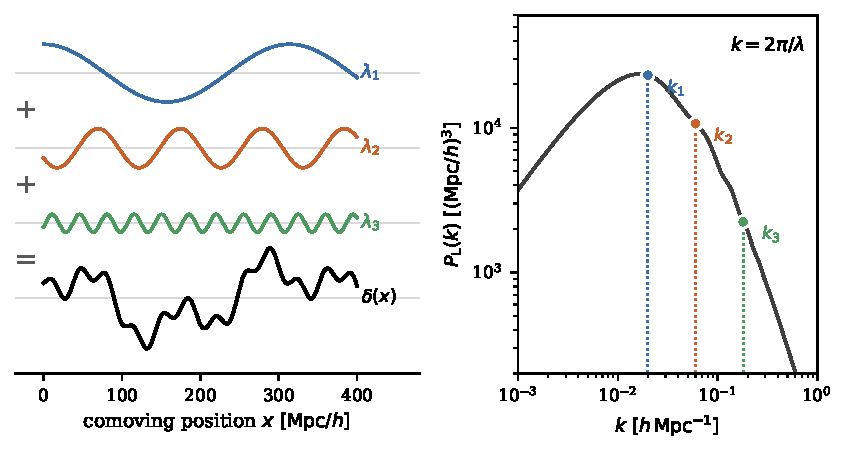
\includegraphics[width=0.96\textwidth]{fourier_decomposition.pdf}
\caption{The same field, held two ways. \emph{Left:} three plane waves of
comoving wavelength $\lambda = 2\pi/k$, added into a lumpy density field
$\delta(x)$. This is a one-dimensional slice for legibility; the real field is
three-dimensional and each mode carries a direction $\khat$ as well as a
wavelength. \emph{Right:} where those same three modes sit on the linear power
spectrum, which is nothing more exotic than amplitude against scale (defined
properly in Section~\ref{sec:stats}, and computed in Section~\ref{sec:linearpk}).
Colours identify the same mode across the two panels.
\newline
One warning, because the picture invites the wrong conclusion. The longest wave
is drawn with the largest amplitude, correctly: a single mode's amplitude goes
as $\sqrt{\Plin(k)}$, and $\Plin$ falls beyond its peak. But that is \emph{not}
the same as large scales dominating the lumpiness. Short-wavelength modes are
far more numerous, and the fluctuation power per logarithmic interval,
$\Delta^2(k) = k^3\Plin(k)/2\pi^2$, rises steeply across these three modes ---
$0.009$, $0.12$, $0.66$. Small scales carry more, which is why nonlinearity
reaches them first, and why almost everything difficult in this course happens
at large $k$.}
\label{fig:fourier}
\end{figure}

\subsection{Why Newtonian dynamics, and which \texorpdfstring{$\delta$}{delta}}
\label{sec:bridge}

Newtonian gravity is two statements: particles fall down a potential,
$\ddot\vx = -\nabla\Phi$, and the potential is sourced by density,
$\nabla^2\Phi = 4\pi G\rho$. Recovering each from general relativity takes a
\emph{different} limit, and it is worth seeing which is which.

\paragraph{Why Fourier, for the dynamics.} Of the two pictures, the linear
problem wants the second one, and not merely for convenience. The linearized
equations are linear with coefficients that do not depend on position --- the
background is homogeneous --- so a plane wave stays a plane wave, and each
$\delta(\vk)$ evolves independently of every other. One partial differential
equation in three dimensions becomes one ordinary differential equation per
$\vk$. That is what makes linear theory solvable at all, and losing it is what
makes everything afterwards hard: nonlinear terms couple modes together, and
organising that coupling is the business of Section~\ref{sec:ept} onwards.

One point about the label. Because $\vk$ is comoving it is fixed once and for
all; it does not change as the universe expands, and what grows is the physical
wavelength $a\lambda$. Nothing in the next paragraph happens because a mode
changes. It happens because the horizon does.

\paragraph{The horizon.} Write $\cH \equiv \dd\ln a/\dd\tau = aH$, the expansion
rate in conformal time --- not the Hubble parameter $H \equiv \dd\ln a/\dd t$.
(Overdots in these notes are $\partial/\partial\tau$ throughout, so $\dot a/a$ is
$\cH$, not $H$. It is also why the growth equation \eqref{eq:growth} below
carries $\cH\dot D$ where its cosmic-time form carries $2H\,\dd D/\dd t$.)
Because $\cH$ is a
\emph{logarithmic} rate --- the fractional growth of $a$ per unit conformal time
--- its definition rearranges to $\Delta\tau = \Delta\ln a/\cH$. One e-fold means
$\Delta\ln a = 1$, so $1/\cH$ is the conformal time in which $a$ grows by a
factor $e$: exactly if $\cH$ held still, and to a factor of order one otherwise
($1.7/\cH$ in radiation domination, $1.3/\cH$ in matter domination; exactly
$1/\cH$ only in de Sitter, where $\cH$ really is constant). Since light moves at
unit comoving speed in conformal time, that same number is the comoving distance
light covers while it happens: the comoving Hubble radius. A time interval and a
length, one number. Loosely, ``the horizon''; strictly it is the Hubble radius, not
the particle horizon $\int\!\dd t/a = \tau$, though in power-law eras the two
agree to a factor of order one ($1/\cH = \tau$ in radiation domination,
$\tau/2$ in matter domination). A mode of comoving wavenumber $k$ is
\emph{sub-horizon} when $k \gg \cH$, meaning its wavelength is short compared
with $1/\cH$, and \emph{super-horizon} when $k \ll \cH$. Inside the horizon a
signal crosses the perturbation many times per expansion time, so gravity and
pressure act coherently across it and local physics is meaningful. Outside,
nothing propagates across the mode at all. You have met the comoving Hubble radius before, running the other way. During
inflation it \emph{shrinks}, which is how modes exit and how their fluctuations
are frozen in as initial conditions. Afterwards it grows, through radiation and
matter domination alike, so a given $k$ starts super-horizon and \emph{enters}
the horizon when $k = \cH$. That is the decisive event in the life of a mode:
what happens to it depends almost entirely on when it entered, which is what the
transfer function of Section~\ref{sec:linearpk} records.

\paragraph{The metric.} Fix the gauge completely with the conformal Newtonian
(longitudinal) form \cite{MaBertschinger1995},
\begin{equation}
\dd s^2 = a^2(\tau)\left[-(1+2\psi)\,\dd\tau^2 + (1-2\phi)\,\delta_{ij}\,\dd x^i\dd x^j\right] .
\label{eq:newtonian_gauge}
\end{equation}
Here $\psi$ perturbs $g_{00}$ and $\phi$ perturbs the spatial metric. Keep them
apart for the moment: the two limits below use different ones, which is the
point.

\paragraph{First limit: slow motion gives the force law.} For a particle with
$v \ll 1$, the geodesic equation in the metric \eqref{eq:newtonian_gauge}
reduces to
\begin{equation}
\ddot\vx + \cH\,\dot\vx = -\nabla\psi
\label{eq:newtonian_eom}
\end{equation}
(Exercise~\ref{ex:geodesic}), which is Newton's second law in comoving
coordinates, with $\cH\dot\vx$ the drag from expansion. So $\psi$, the
perturbation to $g_{00}$, \emph{is} the Newtonian potential. Note what was
required: only that the matter moves slowly. Nothing about $k$.

\paragraph{Second limit: sub-horizon gives the field equation.} The horizon
enters through the field equation instead. One linearized Einstein equation is
the energy constraint \cite[Eq.~(23a)]{MaBertschinger1995},
\begin{equation}
\underbrace{k^2\phi}_{\text{sub-horizon}} +
\underbrace{3\cH\big(\dot\phi + \cH\psi\big)}_{\text{super-horizon}}
= -4\pi G a^2\bar\rho\,\delta .
\label{eq:energy_constraint}
\end{equation}
For $k \gg \cH$ the second group is smaller than the first by $(\cH/k)^2$ and
drops, leaving $-k^2\phi = 4\pi Ga^2\bar\rho\,\delta$: the Poisson equation.
Super-horizon it is the other way round, and there is no Poisson equation to be
had.

Two limits, two jobs --- and two \emph{different} potentials. Slow motion gives
the force law, sourced by $\psi$; sub-horizon gives the field equation, obeyed
by $\phi$. Newtonian gravity has only one potential, so the last thing needed is
that these coincide. They do whenever the total anisotropic stress vanishes
\cite[Eq.~(23d)]{MaBertschinger1995}, which holds for CDM and baryons in the
matter era; free-streaming neutrinos spoil it at the $15\%$ level during
radiation domination, but that contribution fades as matter comes to dominate.
Setting $\phi = \psi \equiv \Phi$ then closes the system --- and two of its three
equations are already in hand. Write the velocity field as $\vu = \dot\vx$ and
its divergence as $\theta \equiv \nabla\cdot\vu$. At linear order the derivative
along a trajectory reduces to $\partial_\tau$, since the advective piece
$\vu\cdot\nabla$ acting on a first-order quantity is second order, so the force
law \eqref{eq:newtonian_eom} is already a field equation; taking its divergence
and substituting the Poisson equation gives the second line below. The third
line \emph{is} the sub-horizon limit of \eqref{eq:energy_constraint}. Only the
first is genuinely new, and it is bookkeeping rather than dynamics --- linearized
mass conservation, whose relativistic dilation term $3\dot\phi$ drops by the same
$(\cH/k)^2$:
\begin{equation}
\dot\delta = -\theta,
\qquad
\dot\theta = -\cH\,\theta - \frac{3}{2}\Om(\tau)\cH^2\delta,
\qquad
\nabla^2\Phi = \frac{3}{2}\Om(\tau)\cH^2\delta ,
\label{eq:newtonian_linear}
\end{equation}
with $\vu \equiv \dd\vx/\dd\tau$,
$\theta \equiv \nabla\cdot\vu$, and $4\pi Ga^2\bar\rho = \tfrac32\Om\cH^2$.

\paragraph{Which \texorpdfstring{$\delta$}{delta}.} One more thing is settled by
$k \gg \cH$, and it is the one students are usually not told. Relativistically
$\delta$ is not a physical quantity: it depends on how spacetime is sliced. The
same mode grows as $(k\tau)^2$ in synchronous gauge and sits frozen in the
Newtonian gauge until horizon entry \cite[\S 7]{MaBertschinger1995} --- which is
why ``do perturbations grow outside the horizon?'' has no gauge-independent
answer. Sub-horizon that ambiguity is suppressed by the same $(\cH/k)^2$, and
$\delta$ becomes something unambiguous to compute, correlate and measure. Every
power spectrum in these lectures stands on that.

\paragraph{Why the metric stays linear.} One consequence of the Poisson equation
is worth drawing out now, because everything after this lecture depends on it.
Inverting $-k^2\Phi = 4\pi Ga^2\bar\rho\,\delta$ gives
\begin{equation}
|\Phi| \sim \frac{3}{2}\,\Om\left(\frac{\cH}{k}\right)^{\!2}\delta ,
\label{eq:phi_small}
\end{equation}
so the potential is the density contrast suppressed by two powers of $\cH/k$ ---
the same factor that licensed the Newtonian limit. At
$k = 0.1\,h\,{\rm Mpc}^{-1}$ that suppression is about $10^{-5}$, so even a patch
with $\delta \sim 100$ carries $|\Phi| \sim 5\times10^{-4}$. Gravity stays weak
precisely where clustering becomes strong.

This is the licence for the rest of the course. We will let $\delta$ grow to
order unity and beyond, and resum it to all orders through loops and
displacements, while never going past linear order in the metric. Those two
statements sound contradictory and are not: $\Phi$ and $\delta$ are separated by
$(\cH/k)^2$, and it is $\delta$ alone that becomes large.

\begin{remark}
The window, then. It closes below at $k\sim\cH$, in practice
$k \sim 10^{-3}\,h\,{\rm Mpc}^{-1}$, where relativistic corrections and the gauge
question both return \cite{Huterer2023}. It does \emph{not} close from pressure:
the post-recombination Jeans scale corresponds to a mass of order
$10^5\,M_\odot$, far below anything here, so cold and pressureless is safe. What
closes it from above is nonlinearity, and two distinct things fail at different
points. The \emph{linearization} goes first, near
$k\sim0.1\,h\,{\rm Mpc}^{-1}$; \eqref{eq:newtonian_linear} is the linearized form
of equations that are themselves nonlinear, and recovering those is the next
section's business. The \emph{Newtonian description} survives further but not
indefinitely, and where it fails is what Lecture~2 is about.
\end{remark}

\subsection{The Vlasov equation and the pressureless fluid}
\label{sec:vlasov}

We now set up the nonlinear problem in the Newtonian regime, following \cite[\S 2]{Bernardeau2002}. Particles obey \eqref{eq:newtonian_eom}, with $\Phi$ the peculiar potential of \eqref{eq:newtonian_linear}. Collisionless matter is then described by its phase-space density $f(\vx,\vp,\tau)$, with $\vp = am\vu$; phase-space conservation gives the Vlasov equation,
\begin{equation}
\frac{\partial f}{\partial\tau} + \frac{\vp}{ma}\cdot\nabla f - am\,\nabla\Phi\cdot\frac{\partial f}{\partial\vp} = 0 .
\label{eq:vlasov}
\end{equation}
Taking velocity moments produces a hierarchy: the zeroth moment gives continuity, the first gives the Euler equation, and each couples to the next through the velocity-dispersion tensor $\sigma_{ij} \equiv \langle u_iu_j\rangle_p - \langle u_i\rangle_p\langle u_j\rangle_p$, where $\langle\cdot\rangle_p$ denotes the momentum average over $f$ at fixed $(\vx,\tau)$ (not the ensemble average of Section~\ref{sec:stats}):
\begin{align}
\dot\delta + \nabla\cdot\left[(1+\delta)\,\vu\right] &= 0 ,
\label{eq:continuity}\\
\dot{\vu} + \cH\,\vu + (\vu\cdot\nabla)\,\vu &= -\nabla\Phi - \frac{1}{\rho}\,\nabla_j\!\left(\rho\,\sigma_{ij}\right).
\label{eq:euler}
\end{align}
Cold matter starts cold: before orbits cross, each position hosts a single stream and $\sigma_{ij} = 0$. This \emph{single-stream closure} truncates the hierarchy into a pressureless perfect fluid. It is a closure rather than a controlled approximation: exact until shell crossing, and completely wrong after. Where it fails is where the effective theory of Lecture~2 will operate.

Within the closure, vorticity $\bm{w} = \nabla\times\vu$ obeys a homogeneous equation: it decays as $1/a$ at linear order and stays zero if it starts zero. The velocity field is then fully specified by its divergence $\theta = \nabla\cdot\vu$.

Linearizing \eqref{eq:continuity}--\eqref{eq:euler} recovers \eqref{eq:newtonian_linear}, which combine into
\begin{equation}
\ddot D + \cH\,\dot D - \frac{3}{2}\Om(\tau)\,\cH^2 D = 0 .
\label{eq:growth}
\end{equation}
The growing solution $D_+(\tau)$ defines linear growth, $\delta^{(1)}(\vx,\tau) = D_+(\tau)\,\delta_0(\vx)$; in Einstein--de Sitter (EdS, $\Om = 1$) $D_+ = a$ and the decaying mode is $a^{-3/2}$. The velocity follows from continuity, and introduces the growth rate $f$ (not to be confused with the phase-space density of \eqref{eq:vlasov}, the one unfortunate collision in the standard notation),
\begin{equation}
\theta^{(1)} = -\cH f\,\delta^{(1)},
\qquad
f \equiv \frac{\dd\ln D_+}{\dd\ln a}
\simeq \Om^{5/9}(\tau) \quad\text{(flat \lcdm)} ,
\label{eq:growth_rate}
\end{equation}
with $f = 1$ in EdS. The often-quoted exponent $0.55$~\cite{Linder2005} agrees with $5/9$ at the sub-percent level over viable cosmologies. The growth rate will return as the central quantity of redshift-space distortions in Lecture~3.

\subsection{Gaussian random fields and the power spectrum}
\label{sec:stats}

Inflation delivers, to very good approximation, Gaussian initial conditions: the linear field $\delta^{(1)}(\vk)$ is a Gaussian random field, meaning that any finite set of its Fourier modes is jointly Gaussian with zero mean. Such a field is characterized completely by its power spectrum,
\begin{equation}
\langle \delta^{(1)}(\vk)\,\delta^{(1)}(\vk')\rangle = (2\pi)^3\dirac(\vk+\vk')\,\Plin(k) ,
\label{eq:plin_def}
\end{equation}
where two distinct assumptions are at work. Statistical \emph{homogeneity} --- invariance under translations --- is what forces the delta function, so that modes whose wavevectors do not sum to zero are uncorrelated. Statistical \emph{isotropy} is a separate statement, invariance under rotations, and it is what makes $\Plin$ a function of the magnitude $k=|\vk|$ alone rather than of the vector $\vk$. Note the one pair that is exempt: $\vk' = -\vk$, where the delta function fires. Since the field is real, $\delta(-\vk) = \delta(\vk)^*$, so that case is $\langle|\delta(\vk)|^2\rangle$ --- a variance, and necessarily non-negative. It is not a counterexample to ``uncorrelated'' but the definition of $\Plin$ itself.

That a Gaussian field is specified completely by $\Plin$ is a practical statement as much as a formal one. To \emph{generate} a realization you draw each Fourier mode independently, with variance $\Plin(k)$ and a random phase, and transform back. That is the first step of any initial-conditions code, and the first step of the hands-on session. Lecture~2 will need the higher moments as well; those are the subject of Section~\ref{sec:wick}.

\subsection{The linear matter power spectrum}
\label{sec:linearpk}

The linear evolution across horizon entry and the radiation--matter transition is what a Boltzmann code integrates. Its output is summarized by the transfer function: modes with $k > k_{\rm eq}$ entered the horizon during radiation domination, when CDM perturbations could barely grow (the M\'esz\'aros effect), so they carry a suppression that larger-scale modes escape. Modes entering after equality avoid it and, once sub-horizon in matter domination, grow approximately as $a$. (Note the care needed after the Comment in Section~\ref{sec:bridge}: a mode that is still super-horizon is \emph{not} growing as $a$ in the Newtonian gauge.) The value $k_{\rm eq} \simeq 0.015\,h\,{\rm Mpc}^{-1}$ is fiducial --- it depends on $\Om h^2$ and on the radiation density. The processed spectrum, including the baryon acoustic oscillation (BAO) wiggles imprinted by the pre-recombination photon--baryon fluid, is what fixes the shape of the $\Plin(k,z)$ defined in \eqref{eq:plin_def}. Everything in these lectures takes $\Plin$ as the input.

\subsection{The Lagrangian picture and the Zel'dovich approximation}
\label{sec:lpt}

How does gravitational collapse actually proceed? A slightly overdense region decelerates the matter around it; particles drift toward it, overshoot, and eventually orbit. The natural variable for this story is not the density at a fixed point but the trajectory of each mass element. Label each fluid element by its initial comoving position $\vq$ and track its displacement,
\begin{equation}
\vx(\vq,\tau) = \vq + \vPsi(\vq,\tau),
\qquad \vPsi(\vq,0)=0 .
\label{eq:displacement}
\end{equation}
This is Lagrangian perturbation theory (LPT). The particle equation of motion \eqref{eq:newtonian_eom} governs $\vPsi$; taking its divergence and using the Poisson equation,
\begin{equation}
\nabla_x\cdot\left[\ddot\vPsi + \cH\,\dot\vPsi\right]
= -\,\frac{3}{2}\,\Om(\tau)\,\cH^2\,\delta\big(\vx(\vq,\tau)\big) .
\label{eq:lpt_master}
\end{equation}
The density needs no equation of its own. Mass conservation, $\bar\rho\,\dd^3q = \rho(\vx)\,\dd^3x$, fixes it algebraically from the volume distortion of the map:
\begin{equation}
1 + \delta(\vx,\tau) = \frac{1}{J(\vq,\tau)},
\qquad
J = \det\left(\delta_{ij} + \Psi_{i,j}\right),
\qquad
\Psi_{i,j} \equiv \frac{\partial\Psi_i}{\partial q_j} .
\label{eq:jacobian}
\end{equation}
A volume element that shrinks ($J<1$) is overdense; one that expands is underdense. Because the determinant is nonlinear in $\vPsi$, a displacement of first order generates density perturbations at all orders: low-order LPT resums an infinite subset of Eulerian nonlinearities, the ones associated with moving matter around. The subset is real but restricted --- the Jacobian generates every power of the linear displacement, not every dynamical nonlinearity --- so more orders in density does not mean more dynamical accuracy at all scales.

At first order, \eqref{eq:lpt_master} with $\delta = -\nabla_q\cdot\vPsi^{(1)}$ (from \eqref{eq:jacobian}) says that the divergence of the displacement obeys the linear growth equation \eqref{eq:growth}. Since the flow is irrotational, $\vPsi^{(1)} = -\nabla_q\varphi^{(1)}$ for a Lagrangian potential $\varphi^{(1)}$, and matching to the Eulerian linear density gives
\begin{equation}
\nabla_q\cdot\vPsi^{(1)}(\vq,\tau) = -\,\delta^{(1)}(\vq,\tau)
\qquad\Longleftrightarrow\qquad
\vPsi^{(1)}(\vk,\tau) = \frac{i\vk}{k^2}\,\delta^{(1)}(\vk,\tau) .
\label{eq:za_displacement}
\end{equation}
The \emph{Zel'dovich approximation} (ZA) \cite{Zeldovich1970} takes this linear displacement seriously beyond linear order in the density: move particles on straight lines (in comoving coordinates) and read the density off the Jacobian. Since $\Psi^{(1)}_{i,j}$ is symmetric it can be diagonalized at each $\vq$, with eigenvalues written $-D_+\lambda_1, -D_+\lambda_2, -D_+\lambda_3$, so
\begin{equation}
\delta_{\rm ZA}(\vx,\tau)
= \frac{1}{\left(1-D_+\lambda_1\right)\left(1-D_+\lambda_2\right)\left(1-D_+\lambda_3\right)} - 1 .
\label{eq:za_density}
\end{equation}
Here is the physical picture of structure formation, sketched in Fig.~\ref{fig:collapse}. At each point the initial conditions define three principal axes with collapse strengths $\lambda_1 > \lambda_2 > \lambda_3$. They are generically unequal for a simple statistical reason: the eigenvalues of a random symmetric matrix are almost never degenerate, so perfectly spherical collapse essentially never happens. Collapse happens first along the $\lambda_1$ axis, when $D_+\lambda_1 \to 1$: matter flattens into a sheet, a Zel'dovich \emph{pancake}, and the density formally diverges. That moment, $J \to 0$, is \emph{shell crossing}. Particle trajectories intersect, the map $\vq\mapsto\vx$ stops being invertible, several streams with different velocities coexist at the same point, and both the single-stream description of Section~\ref{sec:vlasov} and the Zel'dovich solution itself stop being valid.

It is worth being clear about what the rest of Fig.~\ref{fig:collapse} is, then. Formally the second factor in \eqref{eq:za_density} vanishes later wherever $\lambda_2>0$, and the third later still wherever $\lambda_3>0$; the sequence sheet $\rightarrow$ filament $\rightarrow$ knot is that ordering of eigenvalue crossings, and nothing more. As a guide to the \emph{morphology} of the cosmic web it is an excellent one, and it is why the ZA predicts the skeleton of that web from the second derivatives of the initial potential alone. As dynamics past the first caustic it is an extrapolation: a Zel'dovich knot is not a halo, and the approximation says nothing about binding, virialization, or the stable orbiting configuration that collapsed matter actually settles into. Getting through shell crossing needs adhesion models, phase-space methods, or $N$-body simulation.

\begin{figure}[t]
\centering
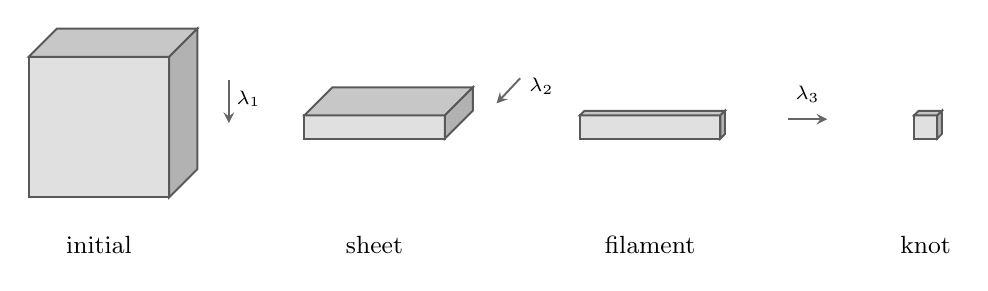
\begin{tikzpicture}[line width=0.7pt, scale=1.0]
% each panel: a box with axis labels, drawn in oblique projection so all three
% axes are visible and each successive collapse is a visible flattening
\newcommand{\panel}[5]{% #1 x-shift, #2 label, #3 sx, #4 sy, #5 sz(depth)
  \begin{scope}[xshift=#1 cm]
    \pgfmathsetmacro{\ax}{1.05*#3}
    \pgfmathsetmacro{\ay}{1.05*#4}
    \pgfmathsetmacro{\dz}{0.42*#5}
    \filldraw[fill=black!12, draw=black!65]
      (-\ax,-\ay) -- (\ax,-\ay) -- (\ax,\ay) -- (-\ax,\ay) -- cycle;
    \filldraw[fill=black!22, draw=black!65]
      (-\ax,\ay) -- (\ax,\ay) -- (\ax+\dz,\ay+\dz) -- (-\ax+\dz,\ay+\dz) -- cycle;
    \filldraw[fill=black!30, draw=black!65]
      (\ax,-\ay) -- (\ax+\dz,-\ay+\dz) -- (\ax+\dz,\ay+\dz) -- (\ax,\ay) -- cycle;
    \node at (0,-1.5) {\small #2};
  \end{scope}}
\panel{0}{initial}{0.85}{0.85}{0.85}
\panel{3.5}{sheet}{0.85}{0.14}{0.85}
\panel{7.0}{filament}{0.85}{0.14}{0.14}
\panel{10.5}{knot}{0.14}{0.14}{0.14}
% collapse arrows, each drawn along the axis that collapses at that step
\draw[->,>=stealth,black!60] (1.65,0.60) -- (1.65,0.05);        % vertical
\node at (1.90,0.36) {\scriptsize $\lambda_1$};
\draw[->,>=stealth,black!60] (5.35,0.62) -- (5.05,0.30);        % into the page
\node at (5.62,0.52) {\scriptsize $\lambda_2$};
\draw[->,>=stealth,black!60] (8.75,0.10) -- (9.25,0.10);        % horizontal
\node at (9.00,0.42) {\scriptsize $\lambda_3$};
\end{tikzpicture}
\caption{The Zel'dovich eigenvalue sequence, drawn in oblique projection so that all three axes are visible. A patch flattens along its principal axes in order of decreasing $\lambda_i$, each stage occurring when the corresponding factor $1-D_+\lambda_i$ in \eqref{eq:za_density} passes through zero: first the vertical axis, giving a sheet, then the depth axis, then the last one --- the second and third only where $\lambda_2$ and $\lambda_3$ are themselves positive, so many patches stop at a sheet. \emph{Only the first crossing is dynamics.} It is a genuine ZA prediction, and it requires a sufficiently positive $\lambda_1$ and enough subsequent growth, so it is not guaranteed at an arbitrary point in a late-time accelerating universe. The second and third stages lie beyond the first caustic, where the approximation has already broken down; read them as the formal eigenvalue ordering, which tracks the morphology of the cosmic web, and not as a description of collapse. The final object is a knot in the deformation map, not a virialized halo.}
\label{fig:collapse}
\end{figure}

\begin{remark}
The ZA is not a degraded linear theory. Its density field \eqref{eq:za_density} contains terms of all orders, and it captures the physics that dominates on quasi-linear scales --- bulk motion --- nonperturbatively. (Exactly, in one dimension before shell crossing, as in Exercise~\ref{ex:1dza}; in three dimensions it is a very good approximation to the displacement, not an exact solution.) This is why the ZA describes the smearing of the BAO feature much better than linear Eulerian theory, why it generates initial conditions for $N$-body simulations, and why its descendants power the infrared resummation of Lecture~3.
\end{remark}

\subsection{Second order: 2LPT and initial conditions}
\label{sec:2lpt}

At second order the displacement responds to the gravitational tide generated at first order. Expanding \eqref{eq:lpt_master} and \eqref{eq:jacobian} to second order, the divergence $\Psi^{(2)}_{i,i}$ obeys the linear-growth operator with a quadratic source \cite[Eqs.~(E.30)--(E.31)]{Jeong2010}; separating variables, the second-order growth factor obeys
\begin{equation}
\ddot D_2 + \cH\dot D_2 - \frac{3}{2}\Om\cH^2 D_2
= -\frac{3}{2}\Om\cH^2 D_+^2 ,
\qquad
D_2(\tau) \simeq -\frac{3}{7}\,D_+^2(\tau)\;\Om^{-1/143},
\label{eq:D2}
\end{equation}
where the fit is accurate to $0.6\%$ for flat \lcdm{} and the EdS limit is $D_2 = -\tfrac37 D_+^2$. (This Lagrangian $D_2$ is a different object from the Eulerian second-order amplitude we will meet in Section~\ref{sec:ept}; the literature uses the same symbol for both.) The spatial source is the second principal invariant of the deformation tensor $\varphi^{(1)}_{,ij}$: writing $\vPsi^{(2)} = \nabla_q\varphi^{(2)}$,
\begin{equation}
\nabla_q^2\varphi^{(2)}
\simeq -\frac{3}{7}\,\Om^{-1/143}
\sum_{i>j}\Big[\varphi^{(1)}_{,ii}\,\varphi^{(1)}_{,jj} - \big(\varphi^{(1)}_{,ij}\big)^2\Big],
\label{eq:2lpt_potential}
\end{equation}
with $\vPsi^{(1)} = -\nabla_q\varphi^{(1)}$ and $\nabla^2_q\varphi^{(1)} = \delta^{(1)}$, both understood as full-time fields with their growth factors included. Do not read \eqref{eq:2lpt_potential} as a purely tidal source: the invariant decomposes into an isotropic piece built from $\delta^2$ and a trace-free tidal piece, and it is nonzero even for a spherical patch, as Exercise~\ref{ex:d2} makes explicit. The full 2LPT map, including velocities, is
\begin{equation}
\vx = \vq - \nabla_q\varphi^{(1)} + \nabla_q\varphi^{(2)},
\qquad
\vu = -\cH f_1 \nabla_q\varphi^{(1)} + \cH f_2\nabla_q\varphi^{(2)},
\qquad
f_2 \simeq 2\,\Om^{6/11} ,
\label{eq:2lpt_map}
\end{equation}
where $f_1 \equiv \dd\ln D_+/\dd\ln a = f$ and, because the convention here has $D_2<0$ so that $\ln D_2$ is undefined,
\begin{equation}
f_2 \equiv \frac{\dd\ln|D_2|}{\dd\ln a} = \frac{\dot D_2}{\cH D_2} .
\label{eq:f2_def}
\end{equation}
The velocity in \eqref{eq:2lpt_map} is unaffected by this: the sign of $D_2$ already sits in $\varphi^{(2)}$. Physically: Zel'dovich streams are straight; the tide bends them. 2LPT is the standard for setting up initial conditions of $N$-body simulations: starting from the ZA alone leaves slowly decaying transients, and 2LPT strongly suppresses them. How large the residual is depends on the starting redshift, the force resolution, and which statistic you look at \cite[App.~E.5]{Jeong2010}.

\begin{remark}
Sign conventions differ across the literature: here $D_2<0$ and the map carries $+\nabla_q\varphi^{(2)}$ \cite[App.~E]{Jeong2010}; other references absorb the minus sign into $D_2$. Check before comparing codes.
\end{remark}

Do the Lagrangian and Eulerian descriptions carry the same information?
Section~\ref{sec:lpt_ept} answers yes, explicitly, once the Eulerian kernels
are in hand.

\begin{exercise}\label{ex:geodesic}
Derive \eqref{eq:newtonian_eom}: write the geodesic equation for a nonrelativistic particle in the metric \eqref{eq:newtonian_gauge}, keep terms to first order in the potentials and to leading order in $u \ll 1$, and use $\phi = \psi = \Phi$. Careful: conformal time is not an affine parameter.
\end{exercise}

\begin{exercise}\label{ex:subhorizon}
\textbf{The other limit.} Exercise~\ref{ex:geodesic} took $v\ll1$ and produced
the force law; this one takes $k\gg\cH$ and produces the field equation.
(i) Reducing \eqref{eq:energy_constraint} to Poisson needs slightly more than
$k\gg\cH$: it needs $\dot\phi$ not to be anomalously large. Assuming
$\dot\phi \lesssim \cH\phi$, which holds for the growing mode, show that the
discarded group is smaller than the retained one by
$\mathcal{O}\big((\cH/k)^2\big)$.
(ii) Put a number on it. Today $\cH_0 = H_0/c \simeq 3.3\times10^{-4}\,h\,{\rm Mpc}^{-1}$.
How large is the neglected term at $k = 0.1\,h\,{\rm Mpc}^{-1}$, and at
$k = 10^{-3}\,h\,{\rm Mpc}^{-1}$? Which of the two lies inside the window quoted
in the Comment above?
(iii) The assumption in (i) can be \emph{removed} rather than justified:
combining the time--time constraint with the time--space one gives an algebraic
equation for $\phi$ carrying no time derivative at all, in which the correction
is manifestly $\mathcal{O}(\cH/k)$ \cite[Ex.~6.7]{DodelsonSchmidt}. Why is
eliminating an assumption preferable to bounding it?
\end{exercise}

\begin{exercise}\label{ex:d2}
Solve \eqref{eq:D2} in EdS ($\cH = 2/\tau$, $\Om=1$, $D_+ = a \propto \tau^2$) and verify $D_2 = -\tfrac37 a^2$.
\end{exercise}

\begin{exercise}\label{ex:1dza}
\textbf{(Optional.)} In one spatial dimension the Zel'dovich approximation is exact until shell crossing. Prove this by showing that the 1D displacement $\Psi^{(1)}$ solves the full nonlinear equation of motion, using the fact that in 1D the force on a sheet depends only on the mass on either side of it. Assume plane-parallel sheets, a subtracted homogeneous background, and boundary conditions (periodic, or a fixed reference point) that determine the constant in $\int\delta\,\dd x$.
\end{exercise}

%=====================================================================
\section*{Lecture 2: From displacements to loops, and where they fail}
\addcontentsline{toc}{section}{Lecture 2: From displacements to loops, and where they fail}
\setcounter{section}{2}
\setcounter{subsection}{0}
\setcounter{equation}{0}
\setcounter{exercise}{0}

\noindent\textbf{Plan (65 min at the board, 25 for questions).} Wick's theorem, and where the loop prefactors come from (0--12) $\rightarrow$ the perturbative kernels, and $F_2$ (12--26) $\rightarrow$ the same $F_2$ recovered from the displacement map you used in the hands-on (26--30) $\rightarrow$ $P_{22}$, $P_{13}$, and the diagrams (30--45) $\rightarrow$ why bare single-stream loops are incomplete (45--51) $\rightarrow$ coarse-graining, the counterterm, and power counting (51--65). \emph{Read, not lectured:} the kernel recursion (Appendix~\ref{app:recursion}) --- $F_2$ is stated and interpreted at the board, not derived; the coarse-grained stress tensor (Appendix~\ref{app:tau}); and most of Section~\ref{sec:eft}, which is the longest section in these notes and the one whose written detail most exceeds its lecture allocation. At the board it is three things only: short modes cannot be computed, their effect on long modes is a $k^2\Plin$ operator with a free coefficient, and fixing that coefficient removes the cutoff dependence (Fig.~\ref{fig:running}). The derivation behind each is here to be read afterwards. Sources:~\cite{Bernardeau2002,BaumannCargese,Baumann2010,Carrasco2012,Carroll2013}.

\subsection{Wick's theorem and the moments of a Gaussian field}
\label{sec:wick}

Everything from here on is built from products of the linear field
$\delta^{(1)}$, whose statistics Section~\ref{sec:stats} fixed. Turning such a
product into a number needs the higher moments of a Gaussian field, and two
facts do all the work.

First, \emph{odd moments vanish}. The Gaussian probability distribution is symmetric under $\delta^{(1)} \to -\delta^{(1)}$, so any average of an odd number of fields is equal to minus itself:
\begin{equation}
\langle \delta^{(1)}_1\,\delta^{(1)}_2\cdots\delta^{(1)}_{2p+1}\rangle = 0 .
\label{eq:odd_vanish}
\end{equation}

Second, \emph{even moments reduce to sums over pairings} (Wick's theorem): an average of $2p$ fields equals the sum, over all ways of dividing the $2p$ fields into $p$ pairs, of the product of two-point functions. The simplest nontrivial case is the four-point function,
\begin{equation}
\langle \delta^{(1)}_1\,\delta^{(1)}_2\,\delta^{(1)}_3\,\delta^{(1)}_4\rangle
= \langle\delta^{(1)}_1\delta^{(1)}_2\rangle\langle\delta^{(1)}_3\delta^{(1)}_4\rangle
+ \langle\delta^{(1)}_1\delta^{(1)}_3\rangle\langle\delta^{(1)}_2\delta^{(1)}_4\rangle
+ \langle\delta^{(1)}_1\delta^{(1)}_4\rangle\langle\delta^{(1)}_2\delta^{(1)}_3\rangle ,
\label{eq:wick4}
\end{equation}
with three pairings. Setting all four fields equal recovers a result you already know for a single Gaussian variable, $\langle x^4\rangle = 3\langle x^2\rangle^2$. In general the number of pairings of $2p$ fields is $(2p-1)!! = (2p-1)(2p-3)\cdots 3\cdot 1$: the first field can pair with any of the $2p-1$ others, the next unpaired field with any of the $2p-3$ remaining, and so on. Counting pairings is how the numerical prefactors of loop calculations arise, as we see next.

\begin{remark}
If the Dirac delta is making the counting hard to see, put the universe in a periodic box of side $L$. The modes are then discrete, $\vk_{\bm{n}} = (2\pi/L)\bm{n}$, and \eqref{eq:plin_def} becomes $\langle\delta_{\bm{n}}\delta_{\bm{m}}\rangle = V\Plin(k_n)\,\delta^{\rm K}_{\bm{n},-\bm{m}}$ with an ordinary Kronecker delta: the average of a product of modes is zero \emph{unless the labels pair up}. Wick's theorem is then the statement that a product of four modes averages to the sum over the three ways of pairing four labels, and each pairing survives only if its two labels are equal and opposite. Every delta function and every combinatorial factor below is that statement in the continuum limit $\sum_{\bm{n}} \to V\!\int\!\dd^3k/(2\pi)^3$.
\end{remark}

Nonlinear evolution makes $\delta$ non-Gaussian, but since $\delta$ will be constructed perturbatively from $\delta^{(1)}$, every statistic reduces to Wick contractions of Gaussian fields. That single fact generates all the loop integrals below.

\subsection{Eulerian perturbation theory}
\label{sec:ept}

In Fourier space the fluid equations \eqref{eq:continuity}--\eqref{eq:euler}, within the single-stream closure of Section~\ref{sec:vlasov}, read \cite[Eqs.~(37)--(39)]{Bernardeau2002}
\begin{align}
\dot\delta(\vk) + \theta(\vk)
&= -\int_{\vk_1}\!\!\int_{\vk_2} (2\pi)^3\dirac(\vk-\vk_{12})\,
\alpha(\vk_1,\vk_2)\,\theta(\vk_1)\,\delta(\vk_2) ,
\label{eq:eom_delta}\\
\dot\theta(\vk) + \cH\,\theta(\vk) + \frac{3}{2}\Om\cH^2\delta(\vk)
&= -\int_{\vk_1}\!\!\int_{\vk_2} (2\pi)^3\dirac(\vk-\vk_{12})\,
\beta(\vk_1,\vk_2)\,\theta(\vk_1)\,\theta(\vk_2) ,
\label{eq:eom_theta}
\end{align}
with $\vk_{12} \equiv \vk_1 + \vk_2$ and the mode-coupling functions
\begin{equation}
\alpha(\vk_1,\vk_2) \equiv \frac{\vk_{12}\cdot\vk_1}{k_1^2},
\qquad
\beta(\vk_1,\vk_2) \equiv \frac{k_{12}^2\,(\vk_1\cdot\vk_2)}{2\,k_1^2k_2^2} .
\label{eq:alpha_beta}
\end{equation}
The function $\alpha$ descends from $\nabla\cdot(\delta\vu)$ in continuity (transport of density by the flow) and $\beta$ from $(\vu\cdot\nabla)\vu$ in Euler (advection of the velocity by itself). Translation invariance forces the convolution structure: two modes couple only into their sum.

Density and velocity are put on the same footing by normalizing the latter. Define the dimensionless velocity divergence
\begin{equation}
\Theta \equiv -\frac{\theta}{\cH f} ,
\label{eq:Theta_def}
\end{equation}
so that \eqref{eq:growth_rate} reads simply $\Theta^{(1)} = \delta^{(1)}$: at linear order the two fields coincide, and any difference between them is purely nonlinear. Every kernel below is a kernel of $\Theta$, never of $\theta$ itself.

In EdS the equations admit a separable solution, each order growing as a power of the growth factor:
\begin{equation}
\delta(\vk,\tau) = \sum_{n\ge1} D_+^n(\tau)\,\delta_n(\vk),
\qquad
\Theta(\vk,\tau) = \sum_{n\ge1} D_+^n(\tau)\,\Theta_n(\vk) ,
\label{eq:eds_ansatz}
\end{equation}
with $D_+ = a$ and $f=1$ in EdS. The time-independent coefficients are convolutions of $n$ copies of the initial field $\delta_0 \equiv \delta^{(1)}/D_+$,
\begin{equation}
\delta_n(\vk) = \int_{\vq_1\cdots\vq_n}
(2\pi)^3\dirac(\vk - \vq_{1\cdots n})\,
F_n(\vq_1,\ldots,\vq_n)\,
\delta_0(\vq_1)\cdots\delta_0(\vq_n) ,
\label{eq:Fn_def}
\end{equation}
and identically for $\Theta_n$ with $F_n \to G_n$. Absorbing the growth factors into the linear fields gives the form the loop integrals actually use,
\begin{equation}
\delta^{(n)}(\vk) = \int_{\vq_1\cdots\vq_n}\!\!(2\pi)^3\dirac(\vk-\vq_{1\cdots n})\,F_n\,
\delta^{(1)}(\vq_1)\cdots\delta^{(1)}(\vq_n) ,
\label{eq:Fn_def_alt}
\end{equation}
and the same with $F_n\to G_n$ for $\Theta^{(n)}$. With this convention the equations of motion reduce to algebraic recursion relations that build $F_n$ and $G_n$ out of $\alpha$, $\beta$, and the lower-order kernels \cite[Eqs.~(43)--(44)]{Bernardeau2002}. They are written out in Appendix~\ref{app:recursion}; all we need here is what they produce. Symmetrizing over the arguments, the second-order kernels are
\begin{equation}
\boxed{\;
F_2(\vq_1,\vq_2) = \frac{5}{7}
+ \frac{1}{2}\frac{\vq_1\cdot\vq_2}{q_1q_2}\left(\frac{q_1}{q_2}+\frac{q_2}{q_1}\right)
+ \frac{2}{7}\frac{(\vq_1\cdot\vq_2)^2}{q_1^2q_2^2},
\qquad
G_2 = F_2\Big|_{\frac57\to\frac37,\ \frac27\to\frac47} .\;}
\label{eq:F2G2}
\end{equation}
The constant term carries isotropic growth, the middle (dipole) term the transport of small-scale structure by large-scale flows, and the last term the tidal coupling.

Some asymptotic properties of the symmetrized kernels organize everything that follows \cite[\S 2.4]{Bernardeau2002}:
\begin{enumerate}[itemsep=1pt,topsep=2pt]
\item \emph{Squeezed total momentum:} as $\vk = \vq_1+\cdots+\vq_n \to 0$ at fixed $\vq_i$, $F_n \propto k^2$. Mass conservation kills the $k^0$ term and momentum conservation the $k^1$ term, so small scales cannot generate large-scale power beyond $k^4$ in the power spectrum (the kernel enters squared).
\item \emph{Hard internal pair:} for $q \gg k$, $F_n(\vq_1,\ldots,\vq_{n-2},\vq,-\vq) \propto k^2/q^2$. UV modes decouple, but only as a power law; this controls how loops respond to small scales.
\item \emph{Single soft leg:} as one $\vq_i \to 0$, $F_n \propto (\vk\cdot\vq_i)/q_i^2$. This infrared enhancement is the advection of small scales by long-wavelength flows; it will cancel in equal-time observables.
\end{enumerate}

Beyond EdS the solutions do not separate exactly: the exact kernels carry weakly time-dependent coefficients multiplying their distinct angular structures. The dependence is weak, but it is not uniform across the kernel. The often-quoted factor $1 + \tfrac{3}{17}(\Om^{-2/63}-1)$, derived for $\Omega_\Lambda = 0$ and below a percent over viable cosmologies \cite[\S 2.4.4]{Bernardeau2002}, applies to the angle-averaged second-order vertex; it is \emph{not} a multiplicative rescaling of $F_2(\vq_1,\vq_2)$ as a whole. Property~3 above shows why it cannot be: the soft limit is fixed exactly by the equivalence principle in every cosmology, so no factor may touch it.

Standard practice, adopted here and in the numerical codes of Lecture~3, is the \emph{EdS-kernel approximation}: keep $F_n$ and $G_n$ at their EdS values and carry all cosmology dependence in $D_+(\tau)$ and $f(\tau)$, i.e.\ evaluate loops with $\Plin(k,z)$. Note what this glosses over --- replacing the exact time dependence of every higher-order velocity kernel by a single power of $f$ --- and that it is an accurate approximation, not an identity.

\subsection{The contact with the Lagrangian picture}
\label{sec:lpt_ept}

The ingredients of $F_2$ were all in place in Lecture~1, in Lagrangian dress.
Making the contact explicit requires one care. Expanding the Jacobian \eqref{eq:jacobian} gives the density as a function of the \emph{Lagrangian} label $\vq$; the Eulerian field at fixed $\vx$ follows from evaluating it at $\vq(\vx) = \vx - \vPsi + \ldots$, which generates an additional transport term at second order:
\begin{equation}
\delta^{(2)}(\vx) = -\Psi^{(2)}_{k,k}
+ \frac12\big(\Psi^{(1)}_{k,k}\big)^2
+ \frac12\,\Psi^{(1)}_{i,j}\Psi^{(1)}_{j,i}
+ \Psi^{(1)}_{j}\,\partial_j\Psi^{(1)}_{k,k} ,
\label{eq:delta2_lpt}
\end{equation}
with all terms on the right evaluated at $\vq = \vx$. Inserting the Fourier-space displacements reproduces the $F_2$ kernel of \eqref{eq:F2G2} (Exercise~\ref{ex:lptf2}); the transport term supplies the dipole. Order by order, before shell crossing, LPT and EPT contain the same information; LPT simply packages it in a variable better adapted to advection.

\subsection{The one-loop matter power spectrum}
\label{sec:1loopmatter}

Insert $\delta = \delta^{(1)} + \delta^{(2)} + \delta^{(3)} + \cdots$ into $\langle\delta\delta\rangle$ and apply the two Gaussian facts of Section~\ref{sec:wick}. Terms with an odd total number of $\delta^{(1)}$'s vanish by \eqref{eq:odd_vanish}: $\langle\delta^{(1)}\delta^{(2)}\rangle$ contains three fields, so it drops. At order $\Plin^2$ two contributions survive, and their prefactors are pure pairing counts:
\begin{itemize}[itemsep=2pt,topsep=2pt]
\item $\langle\delta^{(2)}\delta^{(2)}\rangle$: each $\delta^{(2)}$ contains two linear fields, four in total. Pairing the two fields \emph{inside} the same $\delta^{(2)}$ leaves a contribution at $\vk=0$ only --- a \emph{zero mode}, or tadpole. For matter it vanishes outright, since it is proportional to $F_2(\vq,-\vq) = 0$ (kernel property~1): the dust kernels conserve mass, so $\langle\delta^{(2)}\rangle = 0$ with nothing to subtract. Keep the name anyway, because for biased tracers the analogous term, $\tfrac{b_2}{2}\langle\delta^2\rangle$, is \emph{not} zero and must genuinely be removed --- that is the renormalization of Section~\ref{sec:bias}. The remaining pairings connect the two sides: the first field of the left factor pairs with either field of the right one, and the rest is fixed. \emph{Two} pairings.
\item $\langle\delta^{(1)}\delta^{(3)}\rangle + \langle\delta^{(3)}\delta^{(1)}\rangle$: the external $\delta^{(1)}$ pairs with any of the \emph{three} fields inside $\delta^{(3)}$; the remaining two pair with each other. Three pairings, times two for the two orderings: \emph{six}.
\end{itemize}
Carrying out one of these contractions explicitly shows how the integrals arise. Write both factors using \eqref{eq:Fn_def_alt} and pair $\delta^{(1)}(\vq_1)$ with $\delta^{(1)}(\vq_1')$ and $\delta^{(1)}(\vq_2)$ with $\delta^{(1)}(\vq_2')$. Each pairing supplies one $(2\pi)^3\dirac(\vq_i+\vq_i')\Plin(q_i)$, which removes two of the four momentum integrals. Of the two delta functions from \eqref{eq:Fn_def_alt}, one forces $\vq_1 + \vq_2 = \vk$ and removes a third integral, while the other becomes the overall $\dirac(\vk+\vk')$ that we strip off in defining $P(k)$. A single loop momentum $\vq \equiv \vq_1$ is left free, with $\vq_2 = \vk - \vq$. Both kernels are then evaluated at the same arguments, giving $F_2^2(\vq,\vk-\vq)$, and the two equivalent pairings supply the factor of 2. Written out once, with the delta functions of the two connected pairings visible (the third, disconnected pairing is the $\vk=0$ tadpole just discussed):
\begin{align}
\langle\delta^{(2)}(\vk)\,\delta^{(2)}(\vk')\rangle
&= \int_{\vq_1\vq_2}\!\int_{\vq_1'\vq_2'}
(2\pi)^3\dirac(\vk-\vq_{12})\,(2\pi)^3\dirac(\vk'-\vq_1'-\vq_2')\,
F_2(\vq_1,\vq_2)\,F_2(\vq_1',\vq_2')
\notag\\[2pt]
&\qquad\times
\underbrace{2\,(2\pi)^3\dirac(\vq_1+\vq_1')\Plin(q_1)\;
(2\pi)^3\dirac(\vq_2+\vq_2')\Plin(q_2)}_{\text{Wick: two equivalent pairings}}
\notag\\[2pt]
&= (2\pi)^3\dirac(\vk+\vk')\;\;
2\!\int_{\vq} F_2^2(\vq,\vk-\vq)\,\Plin(q)\,\Plin(|\vk-\vq|) .
\label{eq:p22_derivation}
\end{align}
The two Wick deltas set $\vq_i' = -\vq_i$ and kill the primed integrals; $F_2$ is even, so $F_2(-\vq_1,-\vq_2) = F_2(\vq_1,\vq_2)$; the second kernel delta then reads $\dirac(\vk'+\vq_{12}) = \dirac(\vk'+\vk)$ and is stripped off in defining $P(k)$. Everything else follows the same pattern. The result is
\begin{equation}
P(k,\tau) = \Plin(k,\tau) + P_{22}(k,\tau) + P_{13}(k,\tau) + \mathcal{O}(\Plin^3) ,
\label{eq:P1loop}
\end{equation}
with
\begin{align}
P_{22}(k) &= 2\int_{\vq} \left[F_2(\vq,\vk-\vq)\right]^2
\Plin(q)\,\Plin(|\vk-\vq|) ,
\label{eq:P22}\\
P_{13}(k) &= 6\,\Plin(k)\int_{\vq} F_3(\vk,\vq,-\vq)\,\Plin(q) .
\label{eq:P13}
\end{align}

These expressions have a graphical shorthand, shown in Fig.~\ref{fig:loops}, read with four rules:
\begin{enumerate}[itemsep=1pt,topsep=2pt]
\item every line carries a linear power spectrum $\Plin$ (one line is one Wick pair);
\item every dot (a \emph{vertex}) joining $n$ line ends is a kernel $F_n$;
\item momentum is conserved at each vertex, so a diagram with one closed circuit has exactly one free momentum $\vq$, integrated over as $\int_{\vq}$;
\item the numerical prefactor is the number of Wick pairings that produce the same picture.
\end{enumerate}
The first diagram has no vertex and no closed circuit: it is the linear spectrum itself, called \emph{tree level} because nothing closes back on itself. $P_{22}$ and $P_{13}$ each contain one closed circuit, hence one $\int_{\vq}$: they are the \emph{one-loop} corrections, of order $\Plin^2$. Each extra loop is one extra Wick pair, so two-loop diagrams are of order $\Plin^3$, and so on. The loops here are classical, generated by averaging over random initial conditions, but the bookkeeping is the same as for Feynman diagrams in quantum field theory. One consistency rule matters in practice: contributions of the same order must be kept together. $P_{22}$ without $P_{13}$ is not a meaningful quantity.

\begin{figure}[t]
\centering
\begin{tikzpicture}[line width=0.8pt]
% tree diagram
\draw (-4.7,0) -- (-2.3,0);
\node at (-3.5,0.4) {$\Plin(k)$};
\node at (-3.5,-1.9) {tree};
% P22 diagram
\draw (2,0) circle (1);
\filldraw (1,0) circle (2.2pt);
\filldraw (3,0) circle (2.2pt);
\node at (2,1.32) {$\Plin(q)$};
\node at (2,-1.35) {$\Plin(|\vk-\vq|)$};
\node at (0.62,0) {$F_2$};
\node at (3.38,0) {$F_2$};
\node at (2,-1.9) {$P_{22}$};
% P13 diagram
\begin{scope}[xshift=6.4cm]
\draw (0,0) -- (2.2,0);
\filldraw (2.2,0) circle (2.2pt);
\draw (2.2,0.62) circle (0.62);
\node at (2.2,1.55) {$\Plin(q)$};
\node at (1.1,0.4) {$\Plin(k)$};
\node at (2.2,-0.45) {$F_3$};
\node at (1.1,-1.9) {$P_{13}$};
\end{scope}
\end{tikzpicture}
\caption{Diagrams for the matter power spectrum through one loop. Every line is a linear power spectrum, every dot joining $n$ line ends is the kernel $F_n$, and each closed circuit is integrated over $\vq$. The external mode $\vk$ flows in at one end of the diagram and out at the other; in $P_{22}$ both ends are the vertices themselves.}
\label{fig:loops}
\end{figure}

The two loop contributions play different roles. $P_{22}$ is positive and represents genuine mode coupling: power arrives at $\vk$ from pairs of modes summing to $\vk$. $P_{13}$ is proportional to $\Plin(k)$ and (for CDM-like spectra) negative: it corrects the growth of the existing mode $\vk$, not its shape.

Two structural features of these integrals matter, and they point in opposite directions. The first is already under control, thanks to the displacements of Lecture~1, and returns as a quantitative problem only in Lecture~3. The second is what sets the agenda for the rest of this lecture.

\emph{Infrared.} As $q\to0$ each integrand grows like $\Plin(q)/q^2$, whose integral is the variance of the large-scale velocity (equivalently, of the displacement field of Lecture~1). For spectra with local slope $n_{\rm eff} \equiv \dd\ln\Plin/\dd\ln k \le -1$ the individual integrals are IR divergent, but the divergences cancel in the sum $P_{22}+P_{13}$ \cite[\S 4.2.2]{Bernardeau2002}. The reason is the equivalence principle: a long-wavelength mode displaces everything together, and a uniform displacement cannot change a correlation function evaluated at a single time. (The relevant statement is the cosmological one, sometimes called extended Galilean invariance --- the displacement is time dependent, not a constant-velocity boost.) Exercise~\ref{ex:ir} works this out.

The cancellation is exact, and it is exact whatever the shape of $\Plin$. What it does \emph{not} say is that long modes have no effect. It kills the strictly uniform piece; modes that are soft relative to $k$ but not soft compared with the scale of a feature in the spectrum leave finite, IR-enhanced remainders. For a smooth spectrum those remainders are negligible. For the BAO they are not, and they are what smears the acoustic peak --- the subject of infrared resummation in Lecture~3.

\emph{Ultraviolet.} For $q \gg k$, kernel property 2 gives
\begin{equation}
P_{13}(k) \;\xrightarrow{\ q\gg k\ }\; -\frac{61}{105}\,k^2\,\sigma_v^2\,\Plin(k) ,
\qquad
\sigma_v^2 \equiv \frac{1}{6\pi^2}\int \dd q\,\Plin(q)
\label{eq:P13_UV}
\end{equation}
(the number follows from the angle-averaged limit of the $F_3$ kernel, $-\tfrac{61}{1890}\,k^2/q^2$). The loop responds to all small-scale power through $\sigma_v^2$, including scales where perturbation theory is meaningless. For scale-free spectra $\Plin\propto k^n$ the integral diverges for $n \ge -1$; for a realistic \lcdm{} spectrum it is finite but receives uncontrolled contributions from near the nonlinear scale. The prediction depends on modes we have no right to compute. This is the central failure of the pressureless-fluid loop expansion, and fixing it occupies the rest of this lecture.

\begin{remark}
A useful diagnostic is the dimensionless variance $\Delta^2(k) \equiv k^3P(k)/2\pi^2$, the contribution to $\langle\delta^2\rangle$ per logarithmic interval. Perturbation theory organizes itself in powers of $\Delta^2$: each additional loop costs one power. At the nonlinear scale $\knl$, defined by $\Delta^2(\knl)=1$ (which gives $\knl \simeq 0.25\,h\,{\rm Mpc}^{-1}$ at $z=0$ for the linear spectrum, and is often quoted loosely as $0.2$--$0.3$ depending on the convention), all loops are equally important and the expansion loses meaning.
\end{remark}

\subsection{Why bare single-stream SPT is not a complete long-wavelength theory}
\label{sec:sptfails}

We now have the loop integrals \eqref{eq:P22}--\eqref{eq:P13}. It pays to be precise about what is and is not wrong with them \cite{BaumannCargese,Baumann2010,Carroll2013}, because the loose version of the complaint, that ``SPT has no expansion parameter'', is not true and would contradict the power counting we are about to set up.

\emph{The expansion in the external momentum is fine.} At $k \ll \knl$ the long-wavelength fluctuations really are small, and successive loop corrections really are parametrically suppressed, as the $\Delta^2$ counting of Section~\ref{sec:1loopmatter} says. Nothing is diverging in $k$.

\emph{The internal momenta are the problem.} Each loop integrates over all $q$, including $q \sim \knl$ and beyond, where $\Delta^2(q) \gtrsim 1$ and, more to the point, where the pressureless single-stream equations are not the right equations. So while the \emph{shape} of each loop contribution in $k$ is predicted, part of its \emph{coefficient} is not. The theory returns a definite number, and that number is partly fiction.

\emph{This is not the same thing as a divergence.} Regulating the UV with a cutoff $\Lambda$, the $P_{13}$ integral \eqref{eq:P13_UV} scales as $\Lambda^{n+1}$ for $\Plin \propto k^n$, so it diverges for $n \ge -1$. For a realistic \lcdm{} spectrum, whose effective slope near $\knl$ is steeper than $-1$, the integral converges perfectly well as $\Lambda\to\infty$. A convergent integral that is dominated by a region where your equations are invalid is no more trustworthy than a divergent one; it is just quieter about it.

\emph{And the hard contribution has a predictable form.} Because the kernels decouple as $k^2/q^2$ (property~2), whatever the short scales do reaches long wavelengths analytically in $k$, starting at $k^2\Plin(k)$. That is the structural fact that matters: the damage is confined to a handful of shapes, each of which can be written down as an operator with a free coefficient and fixed by matching. Small-scale physics need not be computed, only parameterized.

\emph{Finally, the fluid closure is genuinely wrong there.} Beyond shell crossing $\sigma_{ij} \neq 0$: multi-streaming generates velocity dispersion and vorticity. Virialized structures do not influence long modes strongly, but they do not decouple exactly either --- their effect is suppressed by powers of $k/\knl$ and by their multipole structure, which is decoupling, not zero.

The resolution is not to push the expansion harder but to change the theory: acknowledge that small scales are not perturbative, remove them, and encode their effect on large scales through the finite set of operators just identified. That is an effective field theory.

\subsection{The effective field theory of large-scale structure}
\label{sec:eft}

Before the formalism, the motivation. A survey of volume $V$ contains $N \sim V k_{\rm max}^3$ independent Fourier modes below $k_{\rm max}$, and statistical errors on the power spectrum shrink as $1/\sqrt{N}$. Doubling the wavenumber reach multiplies the mode count by eight. The EFT program is to push $k_{\rm max}$ as high as possible \emph{while knowing the theoretical error}, so that no bias creeps into the comparison with data \cite{BaumannCargese}.

\subsubsection{Coarse-graining and the effective stress tensor}

Smooth every field over a scale $\Lambda^{-1}$ (that is, average it over spheres of that radius) and split $\delta = \delta_\ell + \delta_s$ into the smoothed long-wavelength part and the short-wavelength remainder. The cutoff $\Lambda$ is a bookkeeping boundary, chosen below $\knl$: modes with $k<\Lambda$ we compute perturbatively; modes above it we do not trust, so their effect must be parameterized. The same $\Lambda$ then bounds the loop integrals, which is why the counterterm below can cancel their cutoff dependence. Smoothing the continuity equation gives back continuity for the long fields, provided the long-wavelength velocity is defined mass-weighted. Smoothing the Euler equation does not close: the quadratic terms leave a remainder sourced by the short modes \cite[App.~A]{Baumann2010},
\begin{equation}
\dot{\vu}_\ell + \cH\vu_\ell + (\vu_\ell\cdot\nabla)\vu_\ell
= -\nabla\Phi_\ell - \frac{1}{\rho_\ell}\,\nabla_j\tau_{ij} ,
\label{eq:smoothed_euler}
\end{equation}
where $\tau_{ij}$, already a coarse-grained object, collects the kinetic and gravitational stresses of the small scales (Appendix~\ref{app:tau}). Coarse-graining \emph{derives} the term that SPT set to zero by hand: the velocity dispersion discarded by the single-stream closure reappears as the influence of unresolved scales on resolved ones.

We cannot compute $\tau_{ij}$, but we do not need to. Split it into its expectation value in the presence of the long-wavelength fields plus a fluctuation,
\begin{equation}
\tau_{ij} = \big\langle\tau_{ij}\big\rangle_{\delta_\ell} + \Delta\tau_{ij} .
\label{eq:tau_split}
\end{equation}
Now be careful about what kind of expansion is available \cite[\S 5]{Baumann2010}. In \emph{space}, yes: the small-scale dynamics has finite spatial extent, of order $\knl^{-1}$, so the response to the long fields is local up to a derivative expansion in $k/\knl$. In \emph{time}, no. The short modes respond over roughly a Hubble time, which is not short compared with the timescale on which the long modes themselves evolve, so the effective stress is generically a functional of the long-wavelength history along the fluid trajectory, not of its instantaneous value. That sounds worse than it is, for a reason the Comment below makes precise. Contracting with $k_ik_j/k^2$ picks out the scalar part, the only piece that couples to $\delta$:
\begin{equation}
\frac{k_ik_j}{k^2}\,\frac{\langle\tau_{ij}\rangle}{\bar\rho}
= c_s^2\,\delta_\ell \;-\; \frac{c_{\rm vis}^2}{\cH}\,\theta_\ell \;+\; \cdots ,
\label{eq:tau_expansion}
\end{equation}
an effective pressure (sound speed) and an effective viscosity, with coefficients set by the small-scale velocity dispersion, plus higher-derivative corrections suppressed by further powers of $k/\knl$. The long-wavelength theory is an \emph{imperfect fluid}, with parameters that cannot be computed within the theory but can be measured, from simulations or from the data itself.

\begin{remark}
This is where the time nonlocality gets absorbed. At the order relevant for the one-loop power spectrum $\delta^{(1)}$ and $\Theta^{(1)}$ are the same field by \eqref{eq:Theta_def}, so the two operators in \eqref{eq:tau_expansion} are degenerate and $c_s^2$, $c_{\rm vis}^2$ enter only through one combination; a time-nonlocal kernel convolved against the long-wavelength history likewise collapses to a single number here, since that history is one growing mode \cite{Carroll2013}. What survives is one effective sound speed, and it is not a physical property of dark matter: it depends on the smoothing scale $\Lambda$, and its value encodes an integral over the past. Treat it as what it is --- the coefficient of an operator, fixed by matching. The degeneracy is a feature of this observable at this order, not a general simplification.
\end{remark}

\subsubsection{The counterterm and renormalization at one loop}

Insert \eqref{eq:tau_expansion} into the equations of motion and solve perturbatively. The coefficient $c_s^2$ is sourced by the small-scale variance, so it is itself of order $\Plin \sim (\delta^{(1)})^2$; multiplying $\delta_\ell \sim \delta^{(1)}$, the new term therefore enters at the same order as $\delta^{(3)}$, producing a \emph{counterterm} correction to the density,
\begin{equation}
\delta_{\rm ctr}(\vk,\tau) = -\,c_s^2(\Lambda,\tau)\,k^2\,\delta^{(1)}(\vk,\tau) ,
\qquad\Longrightarrow\qquad
P_{\rm ctr}(k) = -\,2\,c_s^2\,k^2\,\Plin(k) ,
\label{eq:ctr}
\end{equation}
where $c_s^2$ now denotes the rescaled coefficient, carrying units of $({\rm Mpc}/h)^2$ after absorbing the factors of $\cH$ and the time integrals against growth factors (conventions differ across the literature; this is the one used by the code discussed in Lecture~3 \cite{ClassPT2020}, with the EFT origin in \cite{Baumann2010,Carrasco2012}).

Now compare with the UV limit \eqref{eq:P13_UV} of the loop: $-\tfrac{61}{105}\sigma_v^2(\Lambda)\,k^2\Plin(k)$, with $\sigma_v^2(\Lambda)$ the displacement variance up to the cutoff. The shapes are identical. The cutoff dependence of the loop can therefore be absorbed into the coefficient:
\begin{equation}
P_{\rm 1\text{-}loop}(k)
= \underbrace{P_{22} + P_{13}}_{\text{cutoff-dependent}}
\;\underbrace{-\;2\,c_s^2(\Lambda)\,k^2\,\Plin}_{\text{cancels it}}
\qquad\text{with}\qquad
\frac{\partial\,P_{\rm 1\text{-}loop}}{\partial\Lambda} = 0 .
\label{eq:renormalized}
\end{equation}
This is renormalization, in the same sense as in quantum field theory. Observables cannot depend on the bookkeeping scale $\Lambda$; demanding that they do not fixes how $c_s^2(\Lambda)$ runs, and the leftover finite piece, of order the small-scale velocity dispersion, is the one number the theory cannot predict. One fits it: at $z=0$ the fitted value corresponds to $c_s^2 \sim \mathcal{O}(1)\,({\rm Mpc}/h)^2$ \cite{Carrasco2012}.

Figure~\ref{fig:running} shows this happening. Cutting the loop integrals off at four different $\Lambda$ gives four different predictions, spread by $6.5$ percentage points of $\Plin$ at $k=0.25\,h\,{\rm Mpc}^{-1}$ --- about a tenth of the one-loop correction itself, which is $57\%$ of $\Plin$ there. Fitting one counterterm per cutoff collapses that spread to $0.3$ points. The fitted coefficients are not the same number, and are not supposed to be: they run, and at the rate Exercise~\ref{ex:running} derives. This also settles what the $c_s^2 = 1.1\,({\rm Mpc}/h)^2$ of Fig.~\ref{fig:eftvsspt} means: that calculation regulated nothing, so it is the $\Lambda\to\infty$ member of this family, and the quoted value is not a cutoff-independent property of dark matter.

\begin{figure}[t]
\centering
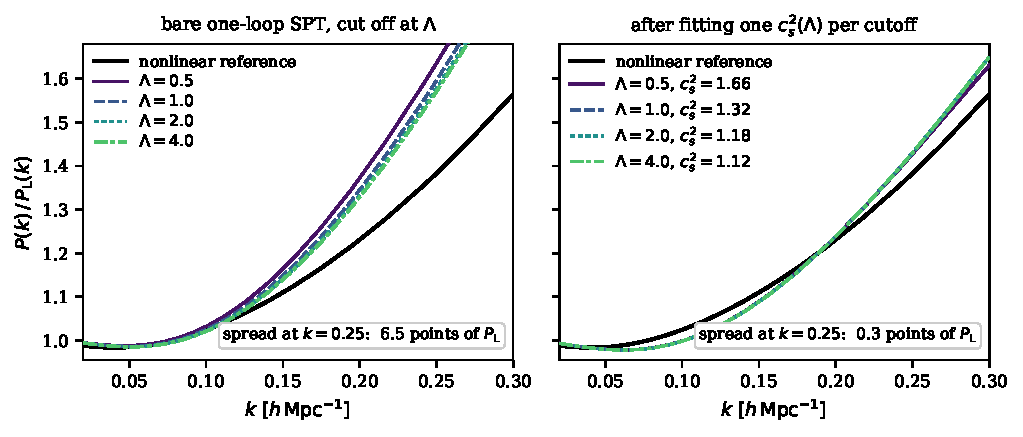
\includegraphics[width=0.94\textwidth]{cutoff_running.pdf}
\caption{Renormalization at work, at $z=0$; no-wiggle input, as in Fig.~\ref{fig:eftvsspt}. \emph{Left:} one-loop SPT with the loop regulated at four cutoffs $\Lambda$, in $h\,{\rm Mpc}^{-1}$. The prediction depends on a scale that is pure bookkeeping, spreading $6.5$ percentage points of $\Plin$ at $k=0.25\,h\,{\rm Mpc}^{-1}$. \emph{Right:} the same four after adding $-2c_s^2(\Lambda)k^2\Plin$, with one $c_s^2$ fitted per cutoff to the halofit reference (heavy black in both panels) over $0.10<k<0.25\,h\,{\rm Mpc}^{-1}$; the spread falls to $0.3$ points, as \eqref{eq:renormalized} demands.
Three caveats, so the figure is not read as proving more than it does. (i) The collapse is measured where the fit was performed, so it is partly guaranteed; beyond the fit range it is $2.0$ points against $7.8$ bare, still a factor of four, and \emph{that} part is not guaranteed. (ii) The cutoff is $\Plin(q)\to\Plin(q)/[1+(q/\Lambda)^{12}]$ rather than a step, so both legs of $P_{22}$ are regulated together; the external $\Plin(k)$ leg of $P_{13}$ is deliberately left unregulated, since only the loop is being cut. The resulting $\sigma_v^2$ matches the sharp-cutoff value to $0.1\%$. (iii) The running comes out as $-0.275, -0.289, -0.290$ for successive cutoff pairs, approaching the $-61/210$ of Exercise~\ref{ex:running} as $\Lambda$ moves deeper into the UV. The trend is the result, not the last number.}
\label{fig:running}
\end{figure}

The stochastic piece $\Delta\tau_{ij}$ in \eqref{eq:tau_split} contributes too, but it is uncorrelated with the long modes: its leading effect on $P(k)$ scales as $k^4$ with no factor of $\Plin$ (kernel property 1: mass and momentum conservation; Exercise~\ref{ex:stoch}), suppressed by additional powers of $k/\knl$ relative to the counterterm for CDM-like spectra. For the matter power spectrum at one loop it can usually be neglected; its analogue for galaxies (shot noise) cannot, as we will see.

\subsubsection{Power counting: ordering the expansion}

The EFT organizes the prediction as a double expansion,
\begin{equation}
P(k) \;=\; \underbrace{\Plin}_{\mathcal{O}(1)}
\;+\; \underbrace{P_{22}+P_{13}}_{\mathcal{O}(\Delta^2)}
\;-\; \underbrace{2c_s^2k^2\Plin}_{\mathcal{O}\left((k/\knl)^2\right)}
\;+\; \underbrace{P_{\rm 2\text{-}loop} + \ldots}_{\mathcal{O}(\Delta^4),\ \ldots}
\label{eq:power_counting}
\end{equation}
in loops (each costs one power of $\Delta^2$) and in derivatives (each counterterm order costs $k^2/\knl^2$). Every term has a definite size at a given $k$, so the expansion can be truncated deliberately: the theoretical error of a truncation is the size of the first omitted term, an estimate you can write down before comparing to anything. This is the practical meaning of a \emph{controlled} expansion: the theory predicts its own error bar, and the fitting range $k_{\rm max}$ is chosen where that error crosses the statistical one.

Figure~\ref{fig:eftvsspt} shows what this buys. Linear theory falls behind the nonlinear reference from $k \approx 0.1\,h\,{\rm Mpc}^{-1}$ onward, reaching a $27\%$ deficit by $k = 0.25\,h\,{\rm Mpc}^{-1}$. One-loop SPT fixes that at first, then overshoots as the uncontrolled UV contribution of \eqref{eq:P13_UV} takes over: it is $8\%$ high at $k=0.20$ and $13\%$ high at $k=0.25\,h\,{\rm Mpc}^{-1}$. One-loop EFT, with a single counterterm fitted over $0.1 < k < 0.25\,h\,{\rm Mpc}^{-1}$, stays close to the reference across that whole range \cite{BaumannCargese,Carrasco2012}. Read the residual with care, though: the counterterm was fitted to this very curve, and halofit is itself a fitting formula good only to a few percent here, so the small differences that remain are not a measurement of how accurate the EFT is. What the figure does support is the failures that are large compared with halofit's own $\sim5\%$ accuracy on these scales \cite{Takahashi2012}: linear theory's $27\%$ deficit and SPT's $13\%$ excess at $k=0.25\,h\,{\rm Mpc}^{-1}$ are real, while SPT's $8\%$ at $k=0.20$ is only about $1.5$ times halofit's own uncertainty and should be read as indicative.

\begin{figure}[t]
\centering
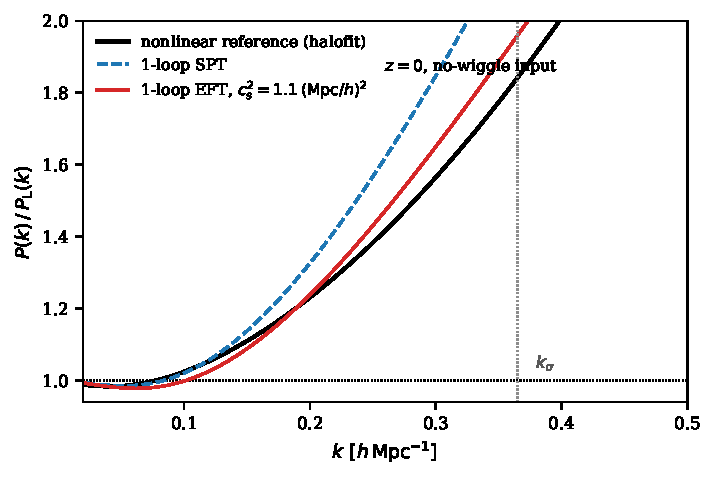
\includegraphics[width=0.70\textwidth]{eft_vs_spt.pdf}
\caption{Matter power spectrum at $z=0$, divided by linear theory. The nonlinear reference is halofit \cite{Takahashi2012}, a formula calibrated to $N$-body simulations; being a fit, it is itself good only to a few percent on these scales, so the comparison is indicative rather than a percent-level validation. One-loop SPT crosses above the reference near $k \approx 0.11\,h\,{\rm Mpc}^{-1}$ and climbs away from it, while one-loop EFT with a single fitted counterterm, $c_s^2 = 1.1\,({\rm Mpc}/h)^2$, stays close. The no-wiggle spectrum \cite{EisensteinHu1998} is used as input so that residual BAO features do not obscure the broadband comparison. The dotted vertical line marks halofit's own nonlinear scale $k_\sigma$, defined by a Gaussian-filtered $\sigma(1/k_\sigma) = 1$; this is a different convention from the $\knl$ of Section~\ref{sec:1loopmatter} and lands at a larger wavenumber.}
\label{fig:eftvsspt}
\end{figure}

\begin{remark}
The counterterm soaks up more than the formal cutoff dependence: it also absorbs the finite error the loop makes in the region $q \sim \knl$, where the pressureless kernels are wrong. That is why the EFT fits simulations better than SPT even when the SPT loop happens to converge. The price is one fitted number per order. But note the limit of this: a counterterm can only absorb contributions whose \emph{shape} lies in the retained operator basis. Missing physics whose $k$ dependence is linearly independent of the retained basis --- non-analyticity being the clearest case --- is not absorbed but mismodelled, and no amount of fitting will reveal that from the fit alone.
\end{remark}

\begin{exercise}\label{ex:f2}
Use the recursions \eqref{eq:Fn_recursion}--\eqref{eq:Gn_recursion} at $n=2$ to derive the unsymmetrized $F_2(\vq_1,\vq_2)$, then symmetrize and verify \eqref{eq:F2G2}. Check two limits: the soft one, $F_2(\vq,\vk-\vq) \to \vk\cdot\vq/(2q^2)$ as $\vq\to0$, in line with kernel property~3; and the zero-total-momentum one, $F_2(\vq,-\vq) = 0$, which is kernel property~1 at $n=2$ and is nothing but mass conservation --- two modes that cancel exactly cannot source a homogeneous overdensity.
\end{exercise}

\begin{exercise}\label{ex:ir}
The infrared cancellation. Using the soft limit from Exercise~\ref{ex:f2}, show that the region $q\to0$ (together with its mirror $|\vk-\vq|\to0$) contributes $P_{22} \supset +\,k^2\sigma_v^2\,\Plin(k)$. The corresponding soft limit of the angle-averaged $F_3(\vk,\vq,-\vq)$ is $-\,k^2/(18q^2)$ (derivable from the recursion, or verifiable numerically), which gives $P_{13} \supset -\,k^2\sigma_v^2\,\Plin(k)$. Conclude that the $\sigma_v^2$ sensitivity cancels in the equal-time sum; compare Table~5 of \cite{Bernardeau2002} (in their conventions). Then argue in words why this exact cancellation of the \emph{strictly} soft contribution does not prevent a feature of intrinsic scale $k_{\rm osc}$ from receiving finite, uncancelled displacement corrections.
\end{exercise}

\begin{exercise}\label{ex:lptf2}
Insert $\vPsi^{(1)}(\vk) = (i\vk/k^2)\delta^{(1)}(\vk)$ and $\vPsi^{(2)}$ from \eqref{eq:2lpt_potential} into \eqref{eq:delta2_lpt}, work in EdS, symmetrize, and recover $F_2$ of \eqref{eq:F2G2}. Identify which term of \eqref{eq:delta2_lpt} produces which piece of $F_2$. (Alternative route: expand the exact map $\delta(\vk) = \int\dd^3q\; e^{-i\vk\cdot\vq}\left(e^{-i\vk\cdot\vPsi(\vq)}-1\right)$ to second order.)
\end{exercise}

\begin{exercise}\label{ex:running}
\textbf{The running of $c_s^2$.} Regulate the loop with a sharp cutoff, so that $\sigma_v^2(\Lambda) = \tfrac{1}{6\pi^2}\int_0^\Lambda\!\dd q\,\Plin(q)$ in \eqref{eq:P13_UV}. Working at order $k^2\Plin(k)$, where $P_{22}$ does not contribute (its leading UV behaviour is $\propto k^4$ with no factor of $\Plin(k)$ --- kernel property 1), impose $\partial P_{\rm 1\text{-}loop}/\partial\Lambda = 0$ from \eqref{eq:renormalized} and derive
\begin{equation*}
\frac{\dd c_s^2}{\dd\ln\Lambda} = -\frac{61}{210}\,\frac{\dd\sigma_v^2}{\dd\ln\Lambda}
= -\frac{61}{210}\,\frac{\Lambda\,\Plin(\Lambda)}{6\pi^2} ,
\qquad\text{so}\qquad
c_s^2(\Lambda) = c_{s,\rm ren}^2 - \frac{61}{210}\,\sigma_v^2(\Lambda) .
\end{equation*}
Then verify that at order $k^2\Plin$ the $\Lambda$ dependence cancels between the two, leaving $-2c_{s,\rm ren}^2k^2\Plin(k)$. (Only at that order: the full $P_{13}$ also contains finite pieces that are not of this shape.) Which part of this is a prediction, and which part is the one number the theory cannot supply? Figure~\ref{fig:running} carries out the corresponding numerical experiment.
\end{exercise}

\begin{exercise}\label{ex:stoch}
\textbf{Why matter stochasticity starts at $k^4$.} A stochastic contribution $\delta_\varepsilon$ to the \emph{matter} density is constrained by conservation laws: mass conservation forces $\int\!\dd^3x\,\delta_\varepsilon = 0$, and momentum conservation forces $\int\!\dd^3x\,x_i\,\delta_\varepsilon = 0$. Argue that these make $\delta_\varepsilon(\vk) = \mathcal{O}(k^2)$ as $k\to0$, hence $P_\varepsilon(k) = \mathcal{O}(k^4)$. Why does the same argument \emph{not} apply to galaxies, whose number is not conserved?
\end{exercise}

%=====================================================================
\section*{Lecture 3: Galaxies in redshift space at one loop}
\addcontentsline{toc}{section}{Lecture 3: Galaxies in redshift space at one loop}
\setcounter{section}{3}
\setcounter{subsection}{0}
\setcounter{equation}{0}
\setcounter{exercise}{0}

\noindent\textbf{Plan (65 min at the board, 25 for questions).} This lecture assembles the model that is actually fit to survey data. The symmetry basis for bias, renormalized operators, stochasticity, higher derivatives (0--20) $\rightarrow$ the redshift-space map, the Kaiser limit, the anatomy of $Z_2$ (20--38) $\rightarrow$ the assembled one-loop spectrum, its counterterm and stochastic sectors, and what IR resummation does to the BAO (38--50) $\rightarrow$ AP, multipoles, and the end-to-end pipeline against real data (50--65). The FFTLog derivation is \emph{not} lectured: Appendix~\ref{app:fftlog} and the companion note \cite{Nguyen2025} carry it, and only the power-law-factorization idea belongs on the board. The six-step recipe at the end is the one part not to skip. Sources: \cite{Desjacques2018,Kaiser1987,ClassPT2020,ChudaykinIvanov2019,IvanovSibiryakov2018,Simonovic2017}.

\subsection{Galaxy bias}
\label{sec:bias}

Surveys measure galaxies rather than matter. Galaxies form in collapsing patches of comoving size $R_*$ over roughly a Hubble time, where $R_*$ is set by the region of the initial field that ends up in one halo (its Lagrangian radius). The galaxy density at $(\vx,\tau)$ is therefore a functional of the matter environment along the past trajectory of the patch. Symmetry fixes what it can depend on \cite[\S 2]{Desjacques2018}. By the equivalence principle, a uniform potential $\Phi$ and a uniform force $\nabla\Phi$ are locally unobservable; both are removed by going to the freely falling frame. The leading locally observable gravitational quantities are the second derivatives $\partial_i\partial_j\Phi$: their trace is the density (via Poisson), their trace-free part is the tidal field. Velocity gradients $\partial_iu_j$ join at the same footing, and by the same argument there is no velocity bias at leading order: galaxies fall like everything else.

The result is the general \emph{bias expansion}: every operator built from $\partial_i\partial_j\Phi$, $\partial_iu_j$, and their time derivatives along the moving patch, with free coefficients. Up to cubic order, which is all that the one-loop power spectrum requires, and in the basis used by the analysis pipelines of this lecture,
\begin{equation}
\boxed{\;
\delta_g = b_1\,[\delta]
+ \frac{b_2}{2}\,[\delta^2]
+ b_{\G_2}\,[\G_2]
+ b_{\Gamma_3}\,[\Gamma_3]
+ \cdots
+ b_{\nabla^2\delta}\,R_*^2\,\nabla^2\delta
+ \varepsilon ,\;}
\label{eq:bias_expansion}
\end{equation}
where square brackets denote \emph{renormalized} composite operators, defined below, and the ellipsis stands for cubic operators ($\delta^3$, $\delta\,\G_2$, $\G_3$) that do not produce independent shapes in the one-loop power spectrum \emph{under the assumptions of these notes} --- they are independent for higher-point functions and for other observables. Here
\begin{equation}
\G_2 \equiv \big(\partial_i\partial_j\Phi_g\big)^2 - \big(\nabla^2\Phi_g\big)^2 ,
\qquad
\Gamma_3 \equiv \G_2(\Phi_g) - \G_2(\Phi_v) ,
\label{eq:G2_Gamma3}
\end{equation}
with $\nabla^2\Phi_g \equiv \delta$ and $\nabla^2\Phi_v \equiv \Theta$ the normalized potentials --- the second being exactly the normalized velocity divergence of \eqref{eq:Theta_def}, which is why that definition was worth making. $\G_2$ is the tidal invariant; $\Gamma_3$, the difference between density- and velocity-derived tides, encodes the memory of gravitational evolution: the two potentials coincide at linear order, so $\Gamma_3$ starts at third order, and it is nonzero there precisely because $\delta^{(2)}$ and $\theta^{(2)}$ are built from the different kernels $F_2$ and $G_2$.

The expansion \eqref{eq:bias_expansion} is completed by three ingredients.

\emph{Renormalization.} Composite operators like $\delta^2$ are not well defined as they stand: $\langle\delta^2\rangle \ne 0$, and its correlation with a long mode contains a loop, $\langle\delta^2(\vk)\,\delta(\vk')\rangle' \supset \tfrac{68}{21}\sigma^2(\Lambda)\Plin(k)$, with $\sigma^2(\Lambda)$ the variance of the linear field at the cutoff: the same shape as linear bias, with a cutoff-dependent amplitude. Subtracting such pieces order by order defines the renormalized operators denoted by square brackets in \eqref{eq:bias_expansion}, and makes $b_1$ the physical large-scale response, $b_1 = \lim_{k\to0} P_{gm}/P_{mm}$, where $P_{gm}$ is the galaxy--matter cross-spectrum and $P_{mm}$ the matter auto-spectrum \cite[\S 2.10]{Desjacques2018}. That identification assumes Gaussian initial conditions and no scale-dependent large-scale response; local primordial non-Gaussianity is the standard counterexample, and it adds operators of its own. All quoted bias values are renormalized ones.

\emph{Higher derivatives.} Galaxy formation is nonlocal in space over $R_*$; Taylor-expanding that nonlocality gives the $\nabla^2\delta$ operator, contributing $-b_{\nabla^2\delta}R_*^2k^2\Plin$ to $P_{gm}$, the same shape as the matter EFT counterterm \eqref{eq:ctr}. Symmetry fixes the operator but neither the size nor the sign of its coefficient, so $b_{\nabla^2\delta}$ is free and may be of either sign; only the product $b_{\nabla^2\delta}R_*^2$ is meaningful, and it is often written as a single dimensionful parameter. The scale $k \sim 1/R_*$ bounds the bias expansion in principle, analogous to $\knl$ for matter. Note that this spatial nonlocality is a separate matter from the nonlocality \emph{in time} along the past trajectory, which is what $\Gamma_3$ encodes and which need not be short compared with $\cH^{-1}$.

\emph{Stochasticity.} Small-scale initial conditions in different patches are uncorrelated with the long modes, so the mapping has a random component $\varepsilon$ with
\begin{equation}
\langle\varepsilon(\vk)\,\varepsilon(\vk')\rangle'
= P_\varepsilon^{\{0\}} + P_\varepsilon^{\{2\}}k^2 + \mathcal{O}(k^4),
\label{eq:stochastic}
\end{equation}
written as an additive expansion because the two coefficients are independent parameters: $P_\varepsilon^{\{2\}}$ need not scale with $P_\varepsilon^{\{0\}}$. The constant $P_\varepsilon^{\{0\}} \equiv P_{\rm shot}$ is \emph{shot noise}: galaxies are a discrete sampling of a continuous field, and a finite number density $\bar n_g$ adds white noise to the measured spectrum. The Poisson value $1/\bar n_g$ is only a first guess, since halos cannot overlap (which suppresses it) while they do cluster (which enhances it). In practice $P_{\rm shot}$ is a free parameter. The analyticity of \eqref{eq:stochastic} at low $k$ reflects a finite correlation length for small-scale stochasticity --- different patches are nearly, not exactly, uncorrelated.

\begin{remark}
Bias conventions are a frequent source of confusion. The basis $\{\delta^2, \G_2\}$ used here relates to the $\{\delta^2, K^2\}$ basis of \cite{Desjacques2018} by $\G_2 = K^2 - \tfrac23\delta^2$, so $b_{\G_2} = b_{K^2}$ but $b_2$ shifts: $b_2^{\G} = b_2^{K} + \tfrac43 b_{K^2}$. A quoted $b_2$ is meaningless without its basis. Useful reference values, from the evolution of an initially unbiased tracer (``coevolution''): $b_{\G_2} = -\tfrac27(b_1-1)$ and $b_{\Gamma_3} = \tfrac{23}{42}(b_1-1)$; halos in simulations roughly follow them. In the one-loop power spectrum $b_{\Gamma_3}$ enters only through the combination $b_{\G_2} + \tfrac25 b_{\Gamma_3}$ (while $b_{\G_2}$ also appears on its own), so $b_{\Gamma_3}$ is usually fixed rather than fit.
\end{remark}

\subsection{Redshift-space distortions}
\label{sec:rsd}

Surveys infer radial positions from redshifts, which are contaminated by peculiar velocities. In the plane-parallel approximation with line of sight $\nhat$, the inferred (redshift-space) position is
\begin{equation}
\vsv = \vx + \frac{u_z(\vx)}{\cH}\,\nhat ,
\qquad u_z \equiv \vu\cdot\nhat .
\label{eq:rsd_map}
\end{equation}
Number conservation, $(1+\delta_g^s)\,\dd^3s = (1+\delta_g)\,\dd^3x$, converts this coordinate change into an exact field-level relation \cite{ChudaykinIvanov2019},
\begin{equation}
\delta_g^s(\vk) = \delta_g(\vk)
+ \int \dd^3x\; e^{-i\vk\cdot\vx}
\left[e^{-i\,(k\mu/\cH)\,u_z(\vx)} - 1\right]\left[1+\delta_g(\vx)\right],
\qquad
\mu \equiv \khat\cdot\nhat .
\label{eq:rsd_exact}
\end{equation}
Expanding it defines redshift-space perturbation theory. At linear order the relation $\theta = -f\cH\,\delta$ of \eqref{eq:growth_rate} converts the velocity term into $f\mu^2\delta$, giving the Kaiser result \cite{Kaiser1987}
\begin{equation}
\delta_g^s(\vk) = \left(b_1 + f\mu^2\right)\delta^{(1)}(\vk)
\qquad\Longrightarrow\qquad
P_{gg}^{s,\rm tree}(k,\mu) = \left(b_1 + f\mu^2\right)^2\Plin(k)
\label{eq:kaiser}
\end{equation}
(Exercise~\ref{ex:kaiser}). Infall onto overdensities squashes structures along the line of sight, enhancing power at $\mu^2 > 0$. At this order the quadrupole-to-monopole ratio depends only on $\beta \equiv f/b_1$ (Exercise~\ref{ex:kaiser_multipoles}). Restoring the amplitude, what the linear redshift-space spectrum constrains is the pair $b_1\sigma_8$ and $f\sigma_8$ --- not $b_1$, $f$, and the primordial amplitude separately. It cannot tell a more strongly clustered universe from a more strongly biased tracer. Breaking that degeneracy needs the broadband \emph{shape}, which carries the cosmology, together with a model and an external calibration: in practice a \lcdm{} mapping $f = f(\Om)$, a BBN prior on $\omega_b$, and a fixed primordial tilt. Higher-order statistics add information but do not remove that logical dependence.

Beyond linear order, expanding \eqref{eq:rsd_exact} together with the bias expansion organizes the series as in \eqref{eq:Fn_def_alt}, with kernels $Z_n$ that merge gravity ($F_n$), velocities ($G_n$, plus explicit $f\mu k$ factors from the exponential), and bias:
\begin{equation}
\delta_g^s(\vk) = \sum_{n=1}^{\infty}
\int_{\vk_1\cdots\vk_n}(2\pi)^3\dirac(\vk-\vk_{1\cdots n})\,
Z_n(\vk_1,\ldots,\vk_n)\,
\delta^{(1)}(\vk_1)\cdots\delta^{(1)}(\vk_n) .
\label{eq:Zn_expansion}
\end{equation}
The linear kernel is just the Kaiser factor,
\begin{equation}
Z_1(\vk) = b_1 + f\mu^2 ,
\label{eq:Z1}
\end{equation}
and the higher ones have a fixed anatomy: a gravity piece built from $F_n$ multiplied by $b_1$, a velocity piece built from $G_n$ multiplied by $f\mu^2$, terms carrying explicit factors of $f\mu k$ from expanding the exponential in \eqref{eq:rsd_exact}, and the bias operators. Appendix~\ref{app:zkernels} writes $Z_2$ out in full and points to $Z_3$. Setting $b_1 = 1$ and all other biases to zero yields the matter kernels $Z_n^m$.

The one-loop galaxy power spectrum in redshift space then has the structure of \eqref{eq:P1loop}, with the same Wick pairing counts:
\begin{align}
P_{gg}^{s}(k,\mu) = Z_1^2(\vk)\,\Plin(k)
&+ 2\!\int_{\vq} Z_2^2(\vq,\vk-\vq)\,\Plin(q)\Plin(|\vk-\vq|)
\notag\\
&+ 6\,Z_1(\vk)\,\Plin(k)\!\int_{\vq} Z_3(\vq,-\vq,\vk)\,\Plin(q)
\;+\; \ldots
\label{eq:Pgg_1loop}
\end{align}
The ellipsis holds the EFT completion. Expanding \eqref{eq:rsd_exact} shows that every power of the small-scale velocity arrives with a factor $k\mu/\cH$: velocities act as spatial derivatives along the line of sight. Virialized motions (``fingers of God'') are therefore higher-derivative operators in redshift space, and the counterterm sector generalizes anisotropically \cite{ChudaykinIvanov2019,ClassPT2020},
\begin{equation}
P_{\rm ctr}^{s}(k,\mu)
= -2\left(\tilde c_0 + \tilde c_2\,f\mu^2 + \tilde c_4\,f^2\mu^4\right)k^2\Plin(k)
\;-\; \tilde c\,f^4\mu^4k^4\big(b_1+f\mu^2\big)^2\Plin(k) ,
\label{eq:rsd_ctr}
\end{equation}
where the last term, formally next order, is kept because fingers of God are numerically enhanced: the relevant dispersion scale $\sigma_v$ exceeds the naive $1/\knl$. The stochastic sector likewise becomes anisotropic,
\begin{equation}
P_{\varepsilon}^{s}(k,\mu) = P_{\rm shot} + a_0\,k^2 + a_2\,\mu^2k^2 ,
\label{eq:rsd_stoch}
\end{equation}
with $a_2$ nearly degenerate with $\tilde c$ over the fitted range, so one keeps a subset in practice.

\begin{remark}
Counting powers of $\mu$: the tree term carries $\mu^0$ to $\mu^4$, the loops extend to $\mu^8$. Only even powers appear, a consequence of the $\nhat \to -\nhat$ symmetry of the plane-parallel mapping. This is why the observables of Section~\ref{sec:multipoles} are the even multipoles.
\end{remark}

\subsection{Infrared resummation and the BAO}
\label{sec:ir}

Lecture 2 left the BAO case open. The cancellation there is not in question, but what survives it is finite rather than zero: modes with $q \gtrsim k_{\rm osc}$ are soft relative to $k$ while $q/k_{\rm osc}$ is \emph{not} small --- in practice the damping is built from $q$ several times $k_{\rm osc}$, as the kernel in \eqref{eq:sigma_defs} makes explicit --- so the expansion in $q/k_{\rm osc}$ is not suppressed, and the surviving terms accumulate into a smearing of the peak. Displacements of order $\Sigma \sim$ few Mpc$/h$ blur the BAO feature --- the imprint of the sound horizon at the drag epoch, shortly after photon decoupling, at a comoving separation $r_d \simeq 100\,h^{-1}$Mpc. Figure~\ref{fig:bao} shows the effect. Fixed-order perturbation theory captures this damping only order by order, slowly; the physics (from Lecture~1: the Zel'dovich displacement) can instead be resummed to all orders \cite{Senatore2014,Blas2016,IvanovSibiryakov2018}.

The practical scheme splits the linear spectrum into smooth and wiggly parts, $\Plin = P_{\rm nw} + P_{\rm w}$ (numerically, by filtering the BAO oscillations out of $\ln\Plin$), and damps only the wiggly part with the variance of displacements over separations up to the BAO scale. That scale enters through $k_{\rm osc}$, with $k_{\rm osc}^{-1} \simeq 110\,h^{-1}$Mpc in the convention of \cite{ClassPT2020}: the same sound-horizon scale as $r_d$ above, the small difference being a matter of how the oscillation wavelength is defined. With a separation scale $k_S \simeq 0.2\,h\,{\rm Mpc}^{-1}$ and $j_0$, $j_2$ the spherical Bessel functions,
\begin{equation}
\Sigma^2 = \frac{1}{6\pi^2}\int_0^{k_S}\!\dd q\,P_{\rm nw}(q)
\left[1 - j_0\!\left(\frac{q}{k_{\rm osc}}\right) + 2j_2\!\left(\frac{q}{k_{\rm osc}}\right)\right],
\qquad
\delta\Sigma^2 = \frac{1}{2\pi^2}\int_0^{k_S}\!\dd q\,P_{\rm nw}(q)\,
j_2\!\left(\frac{q}{k_{\rm osc}}\right),
\label{eq:sigma_defs}
\end{equation}
and in redshift space the damping becomes anisotropic \cite[Eqs.~(2.25),~(2.30),~(2.31)]{ClassPT2020},
\begin{equation}
\Sigma^2_{\rm tot}(z,\mu) = \left[1 + f\mu^2(2+f)\right]\Sigma^2(z)
+ f^2\mu^2(\mu^2-1)\,\delta\Sigma^2(z) .
\label{eq:sigma_tot}
\end{equation}
The IR-resummed spectrum at one loop is assembled as
\begin{align}
P_{gg}^{s,\rm IR}(k,\mu)
&= Z_1^2(\vk)\left[P_{\rm nw}
+ e^{-k^2\Sigma^2_{\rm tot}}\big(1+k^2\Sigma^2_{\rm tot}\big)P_{\rm w}\right]
\notag\\
&\quad
+ P_{gg}^{s,\rm 1\text{-}loop}\big[P_{\rm nw}\big]
+ e^{-k^2\Sigma^2_{\rm tot}}
\Big(P_{gg}^{s,\rm 1\text{-}loop}\big[\Plin\big]
- P_{gg}^{s,\rm 1\text{-}loop}\big[P_{\rm nw}\big]\Big) ,
\label{eq:ir_resummed}
\end{align}
where $P^{s,\rm 1\text{-}loop}_{gg}[P]$ denotes the loop formulas evaluated with input spectrum $P$. The factor $(1+k^2\Sigma^2_{\rm tot})$ at tree level subtracts the damping already generated by the one-loop terms, preventing double counting.

Two caveats on \eqref{eq:ir_resummed}. It is the tree-plus-loop \emph{core}, not the complete model: the counterterm \eqref{eq:rsd_ctr} and stochastic \eqref{eq:rsd_stoch} sectors still have to be added, and in production codes the counterterm is built on the resummed spectrum so that its wiggly part is damped too (step~3 of the recipe below). And the factorization is itself an approximation --- terms with multiple wiggly insertions are dropped or approximated, and the result inherits whatever algorithmic uncertainty the wiggle/no-wiggle split carries. Those errors are higher order, but they are real, and $k_S$ is an arbitrary separation scale whose residual effect is a useful implementation check rather than a physical parameter.

\begin{figure}[t]
\centering
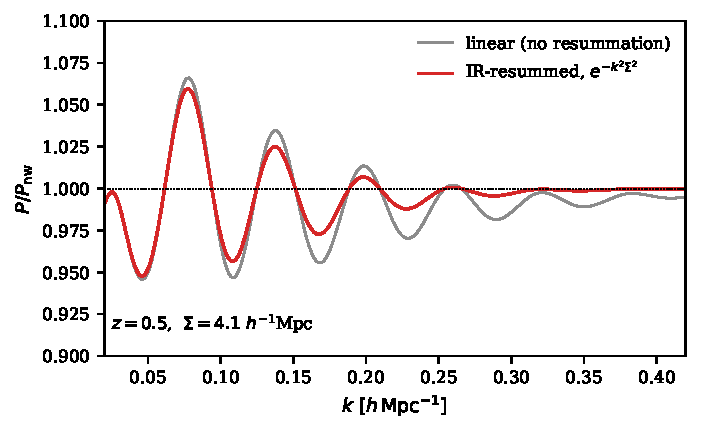
\includegraphics[width=0.68\textwidth]{bao_damping.pdf}
\caption{The BAO feature at $z=0.5$, shown as the ratio of the full spectrum to its smooth part. Bulk flows with $\Sigma \simeq 4\,h^{-1}$Mpc wash out the oscillations progressively toward smaller scales. Linear theory (grey) keeps them at full amplitude; IR resummation (red) damps them as the data require. Plotted for the isotropic damping $e^{-k^2\Sigma^2}$ to keep the figure one-dimensional; in redshift space the exponent carries the $\mu$ dependence of \eqref{eq:sigma_tot}, and the tree-level term the compensating factor of \eqref{eq:ir_resummed}.}
\label{fig:bao}
\end{figure}

\begin{remark}
IR resummation changes no ingredient of the calculation: the same tree and loop building blocks are evaluated with two input spectra and recombined. The damping is nonperturbative information, an all-orders resummation of displacement effects, injected through an exponential. Skipping it misfits the BAO wiggles at a level well above survey precision.
\end{remark}

\subsection{Multipoles, distances, and the parameter set}
\label{sec:multipoles}

The observable spectrum depends on $\mu$ only through even powers; it is compressed into Legendre multipoles,
\begin{equation}
P_\ell(k) = \frac{2\ell+1}{2}\int_{-1}^{1}\dd\mu\;
\mathcal{L}_\ell(\mu)\,P^{s,\rm IR}_{gg}(k,\mu),
\qquad \ell = 0, 2, 4 ,
\label{eq:multipoles}
\end{equation}
with $\mathcal{L}_0 = 1$, $\mathcal{L}_2 = (3\mu^2-1)/2$, $\mathcal{L}_4 = (35\mu^4-30\mu^2+3)/8$. One more step separates theory from data: converting observed redshifts and angles into distances requires assuming a cosmology (the \emph{fiducial} one, subscript ``fid''). If it differs from the true one, wavenumbers are distorted anisotropically, since the radial direction is converted with $H(z)$ and the transverse one with the comoving angular diameter distance $D_M(z) = (1+z)D_A(z)$, which matches the comoving coordinates used throughout. This is the Alcock--Paczynski effect,
\begin{equation}
k_{\rm true}^2 = k_{\rm obs}^2\left[
\frac{H_{\rm true}^2}{H_{\rm fid}^2}\,\mu_{\rm obs}^2
+ \frac{D_{M,\rm fid}^2}{D_{M,\rm true}^2}\big(1-\mu_{\rm obs}^2\big)\right],
\qquad
\mu_{\rm true}^2 = \frac{k_{\rm obs}^2}{k_{\rm true}^2}\,
\frac{H_{\rm true}^2}{H_{\rm fid}^2}\,\mu_{\rm obs}^2 ,
\label{eq:ap}
\end{equation}
which carries the distance information of the BAO scale into the multipoles. The transformation also rescales the overall amplitude by the ratio of survey volumes, $H_{\rm true}D_{M,\rm fid}^2/H_{\rm fid}D_{M,\rm true}^2$; this Jacobian is part of the model. It is $k$- and $\mu$-independent, hence nearly degenerate with the free amplitude, which is why it is easy to forget --- and why forgetting it shows up in $b_1\sigma_8$ and $f\sigma_8$ rather than announcing itself.

The complete one-loop model for one galaxy sample is specified by the cosmology plus the \emph{nuisance parameters} of Table~\ref{tab:params}: quantities we do not care about but must fit alongside the cosmology, since they affect the prediction. A \emph{full-shape} analysis fits the whole measured $P_\ell(k)$ with this model, in contrast to a BAO-only analysis, which uses just the position of the acoustic feature. Analyses of BOSS (the Baryon Oscillation Spectroscopic Survey) fit $\ell = 0, 2$ (and 4) up to $k_{\rm max} \simeq 0.2\,h\,{\rm Mpc}^{-1}$ \cite{Ivanov2020}, guided by comparing the estimated two-loop contribution with the statistical errors \cite{ChudaykinIvanov2019}. That comparison is one input, not the whole procedure: scale cuts are also set by mock validation, estimator systematics, prior sensitivity, and explicit parameter-recovery tests. The organization presented here is one of several in current use --- DESI has compared \texttt{velocileptors}, \texttt{PyBird} and \texttt{FOLPS}-style one-loop EFT models, which share this logic but differ in perturbative organization and nuisance basis \cite{Maus2024,DESI2024V}.

\begin{table}[t]
\centering
\small
\begin{tabular}{llll}
\toprule
Parameter & Role & Illustrative scale (BOSS-like) & Units \\
\midrule
\multicolumn{4}{l}{\emph{Bias: properties of the tracer}}\\
$b_1$ & linear bias & $\approx 2$ & --- \\
$b_2$ & quadratic bias & $\approx -0.6$ & --- \\
$b_{\G_2}$ & tidal bias & $\approx -0.3$; coevolution $-\tfrac27(b_1{-}1)$ & --- \\
$b_{\Gamma_3}$ & cubic (nonlocal-in-time) bias & fixed: $0$ or $\tfrac{23}{42}(b_1{-}1)$ & --- \\
\midrule
\multicolumn{4}{l}{\emph{Derivative and RSD counterterms: degenerate among themselves}}\\
$b_{\nabla^2\delta}R_*^2$ & higher-derivative bias & either sign; degenerate with $\tilde c_0,\tilde c_2$ & $({\rm Mpc}/h)^2$ \\
$\tilde c_0,\ \tilde c_2,\ \tilde c_4$ & counterterms ($\mu^0,\mu^2,\mu^4$) & $\mathcal{O}(10\text{--}30)$ & $({\rm Mpc}/h)^2$ \\
$\tilde c$ & $k^4\mu^4$ finger-of-God term & $\sim\sigma_v^4 \sim 500$ & $({\rm Mpc}/h)^4$ \\
\midrule
\multicolumn{4}{l}{\emph{Stochastic: uncorrelated with the long modes}}\\
$P_{\rm shot}$ & constant stochastic amplitude & $\sim 1/\bar n_g \sim 3\text{--}5\times10^3$ & $({\rm Mpc}/h)^3$ \\
$a_0,\ a_2$ & $k^2$ and $\mu^2k^2$ stochastic terms & often dropped; $a_2$ near-degenerate with $\tilde c$ & $({\rm Mpc}/h)^5$ \\
\bottomrule
\end{tabular}
\caption{Nuisance parameters of the one-loop EFT galaxy power spectrum in redshift space, grouped by what they represent. The numbers are order-of-magnitude scales for one convention (that of \cite{ClassPT2020,ChudaykinIvanov2019}) and one BOSS-like sample at $z\simeq0.5$; they are not universal physical values, and several are strongly convention dependent. The higher-derivative bias is not fitted separately because it is degenerate with the counterterms, but the degeneracy is worth stating correctly: it enters through the linear kernel, $Z_1 = b_1 + f\mu^2 - b_{\nabla^2\delta}R_*^2k^2$, so squaring gives $-2(b_1+f\mu^2)\,b_{\nabla^2\delta}R_*^2k^2\Plin$. That shifts $\tilde c_0$ by $b_1 b_{\nabla^2\delta}R_*^2$ \emph{and} $\tilde c_2$ by $b_{\nabla^2\delta}R_*^2$. It is degenerate with a direction in the counterterm space, not with $\tilde c_0$ alone. Whether the quoted $P_{\rm shot}$ is the full constant or the residual after Poisson subtraction is itself a convention; check before comparing.}
\label{tab:params}
\end{table}

\subsection{Evaluating the loops, and the end-to-end recipe}
\label{sec:fftlog}

One practical obstacle remains. The loop terms in \eqref{eq:Pgg_1loop} are convolution integrals that must be recomputed for every trial cosmology in a parameter scan, and direct numerical integration is far too slow for that. The trick that makes modern analyses possible \cite{Simonovic2017,ClassPT2020} rests on one observation: if the linear spectrum were a pure power law, every loop integral could be done analytically, in closed form in terms of Gamma functions. So one writes $\Plin$ as a sum of (complex) power laws, which is a discrete Fourier transform in $\ln k$, does each integral analytically, and sums. The loop calculation becomes a matrix multiplication with cosmology-independent matrices computed once and for all. Appendix~\ref{app:fftlog} gives the expansion and the master integral; the companion note \cite{Nguyen2025} develops the full hierarchy. This is the algorithm behind \texttt{CLASS-PT} \cite{ClassPT2020} and related codes, and it is why step 2 below costs seconds rather than hours.

Everything is now in place. To confront theory with a measured galaxy power spectrum:
\begin{enumerate}[itemsep=1pt,topsep=2pt]
\item run a Boltzmann code for the trial cosmology to get $\Plin(k,z)$, its growth rate $f(z)$, and the wiggle/no-wiggle split;
\item evaluate the tree and one-loop terms of \eqref{eq:Pgg_1loop} with the FFTLog matrices, for both $\Plin$ and $P_{\rm nw}$;
\item assemble the IR-resummed spectrum \eqref{eq:ir_resummed}, adding the counterterm \eqref{eq:rsd_ctr} and stochastic \eqref{eq:rsd_stoch} contributions with free coefficients;
\item apply the AP conversion \eqref{eq:ap}, including its volume Jacobian, and project onto multipoles \eqref{eq:multipoles};
\item pass the theory multipoles through the \emph{survey measurement operator}: average over the finite $k$ bins, apply the survey window (or the response of a window-deconvolved estimator), and add the integral-constraint and systematic-weight corrections. This is what makes a theory curve commensurable with a data vector; Appendix~\ref{app:window} sketches what it contains;
\item compare $P_{0,2,4}(k)$ with the measurements up to $k_{\rm max}$ and sample the parameters, marginalizing over the nuisance directions rather than fixing them.
\end{enumerate}
The last step is standard statistical inference. The measurements, one number per $k$ bin per multipole, scatter around the truth with a covariance matrix estimated from mock catalogs or from theory, so the probability of the data given a parameter set (the \emph{likelihood}) is approximately a Gaussian in the residual between measurement and model. Multiplying by priors gives the posterior, which is explored by sampling: a Markov chain Monte Carlo (MCMC) walks through the parameter space, visiting each point in proportion to its probability. Projecting the resulting chain onto the cosmological parameters, and ignoring the nuisance directions, automatically accounts for our ignorance of the latter (this is \emph{marginalization}).

Figure~\ref{fig:multipoles} is the end of that road: the assembled one-loop model, everything in this lecture put together, against a synthetic measurement carrying the statistical errors of a BOSS-like volume. The BAO wiggles survive in both multipoles, damped by the IR resummation of Section~\ref{sec:ir}; the quadrupole is positive and comparable to the monopole, the Kaiser signature of infall.

The shaded band is the estimated two-loop contribution, the theoretical error of stopping at one loop. It stays below the statistical errors out to $k \simeq 0.15\,h\,{\rm Mpc}^{-1}$ and overtakes them beyond, which is the quantitative version of the statement that the expansion predicts its own reach. Published analyses fit to $k_{\rm max} \simeq 0.2\,h\,{\rm Mpc}^{-1}$, a little further than this crude comparison suggests, because marginalizing over the nuisance parameters of Table~\ref{tab:params} lets the counterterms absorb part of the missing contribution \cite{ChudaykinIvanov2019,Ivanov2020}.

\begin{figure}[t]
\centering
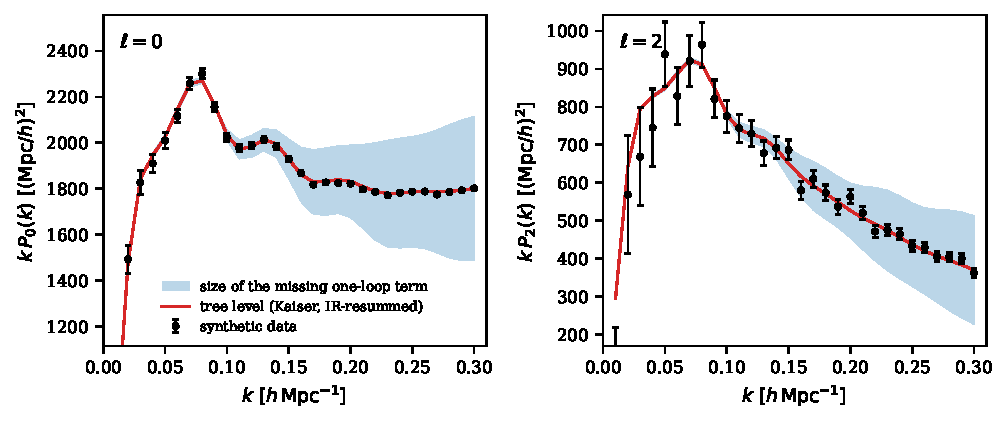
\includegraphics[width=0.94\textwidth]{multipoles.pdf}
\caption{The one-loop EFT galaxy power spectrum in redshift space at $z=0.5$, the model this course has been building. Bias parameters are $b_1 = 2$ with $b_2 = -0.6$ and the coevolution values for $b_{\G_2}$ and $b_{\Gamma_3}$; counterterms and stochastic terms as in Table~\ref{tab:params}. Error bars are for a survey of $6\,(h^{-1}{\rm Gpc})^3$ with $\bar n_g = 3\times10^{-4}\,(h\,{\rm Mpc}^{-1})^3$, and the points are a synthetic realisation scattered by them. The band is the two-loop estimate of \cite{ChudaykinIvanov2019}. Computed with the author's \texttt{FFTLog} implementation, which follows the algorithm of \cite{Simonovic2017,ClassPT2020} and is documented in the companion note \cite{Nguyen2025}.}
\label{fig:multipoles}
\end{figure}

Steps 1--5 take a few seconds per cosmology; that speed is what makes step 6 feasible, since a chain needs many thousands of evaluations. (How many depends strongly on the sampler, on whether the nuisance parameters are marginalized analytically, and on whether gradients or an emulator are available --- modern choices differ by orders of magnitude.) Applied to BOSS data, this pipeline yields constraints on $H_0$, $\Om$, and the clustering amplitude $\sigma_8$ (the rms linear density fluctuation in spheres of $8\,h^{-1}$Mpc) from galaxy clustering that are competitive with those from the cosmic microwave background, and independent of CMB \emph{data} \cite{Ivanov2020}. ``Independent'' is not ``prior-free'': that baseline analysis imposes a BBN prior on $\omega_b$, fixes the primordial tilt $n_s$, and restricts the neutrino sector. Quote the result with its assumptions attached.

\begin{exercise}\label{ex:kaiser}
Derive the Kaiser formula \eqref{eq:kaiser}: expand \eqref{eq:rsd_exact} to linear order, use $u_z(\vk) = -i\mu\,\theta(\vk)/k$ for an irrotational flow, and $\theta = -f\cH\,\delta$.
\end{exercise}

\begin{exercise}\label{ex:z2}
Derive $Z_2$. (i) Check first that setting $f\to0$ in \eqref{eq:Z2} recovers the real-space galaxy kernel $b_1F_2 + \tfrac{b_2}{2} + b_{\G_2}[(\khat_1\cdot\khat_2)^2-1]$. (ii) Then do the work: expand \eqref{eq:rsd_exact} to second order, using $u_z(\vk) = -i\mu\,\theta(\vk)/k$ and $\theta = -\cH f\delta$, symmetrize under $\vk_1\leftrightarrow\vk_2$, and recover every term of \eqref{eq:Z2} --- including each factor of $\tfrac12$, and each power of $f$, $\mu_i$ and $k_i$. You will need the identity $k\mu = k_1\mu_1 + k_2\mu_2$. Say which $\tfrac12$ is a symmetrization and which is a Taylor coefficient.
\end{exercise}

\begin{exercise}\label{ex:kaiser_multipoles}
Project the Kaiser spectrum \eqref{eq:kaiser} onto multipoles and show
$P_0 = \big(b_1^2 + \tfrac23 b_1 f + \tfrac15 f^2\big)\Plin$,
$P_2 = \big(\tfrac43 b_1 f + \tfrac47 f^2\big)\Plin$,
$P_4 = \tfrac{8}{35}f^2\,\Plin$.
\end{exercise}

%=====================================================================
\appendix
\section*{Appendices}
\addcontentsline{toc}{section}{Appendices}
\setcounter{section}{0}
\renewcommand{\thesection}{\Alph{section}}
\setcounter{equation}{0}
\renewcommand{\theequation}{\thesection.\arabic{equation}}

\noindent These collect the derivations and explicit formulae that the lectures
use but do not need to display. The main text can be followed without them; they
are needed to reproduce the numbers, and Exercises~\ref{ex:f2}
and~\ref{ex:z2} send you here directly.

\section{The Eulerian kernel recursion}
\label{app:recursion}

Inserting the EdS ansatz \eqref{eq:eds_ansatz}--\eqref{eq:Fn_def} into the equations of motion
\eqref{eq:eom_delta}--\eqref{eq:eom_theta} and collecting terms of order $n$
gives, at each order, a $2\times2$ linear system for $(F_n, G_n)$ whose solution
is \cite[Eqs.~(43)--(44)]{Bernardeau2002}: with $\vk_1 = \vq_1+\cdots+\vq_m$,
$\vk_2 = \vq_{m+1}+\cdots+\vq_n$ and $F_1 = G_1 = 1$,
\begin{align}
F_n(\vq_1,\ldots,\vq_n) &= \sum_{m=1}^{n-1}
\frac{G_m(\vq_1,\ldots,\vq_m)}{(2n+3)(n-1)}
\Big[(2n+1)\,\alpha(\vk_1,\vk_2)\,F_{n-m}
+ 2\,\beta(\vk_1,\vk_2)\,G_{n-m}\Big] ,
\label{eq:Fn_recursion}\\
G_n(\vq_1,\ldots,\vq_n) &= \sum_{m=1}^{n-1}
\frac{G_m(\vq_1,\ldots,\vq_m)}{(2n+3)(n-1)}
\Big[3\,\alpha(\vk_1,\vk_2)\,F_{n-m}
+ 2n\,\beta(\vk_1,\vk_2)\,G_{n-m}\Big] ,
\label{eq:Gn_recursion}
\end{align}
where $F_{n-m}$ and $G_{n-m}$ carry the arguments $(\vq_{m+1},\ldots,\vq_n)$;
$G_n$ is the kernel of $\Theta$, \eqref{eq:Theta_def}. The recursion produces
\emph{unsymmetrized, ordered} kernels.
The prefactor is what is left of the determinant of that system; it degenerates
at $n=1$, where the growing mode is the homogeneous solution. Kernels are
symmetrized over their arguments before use, meaning averaged over the $n!$
permutations, not summed. Running the recursion at $n=2$ and symmetrizing gives
\eqref{eq:F2G2}.

\section{The coarse-grained stress tensor}
\label{app:tau}

Smoothing the \emph{pressureless-fluid} equations of Section~\ref{sec:vlasov}
over $\Lambda^{-1}$ leaves an effective stress with a kinetic and a
gravitational part, $\tau_{ij} = \tau^{\rm kin}_{ij} + \tau^{\rm grav}_{ij}$
\cite[App.~A]{Baumann2010}. Writing $[X]_\Lambda \equiv W_\Lambda * X$ for the
smoothing, and defining the long-wavelength velocity \emph{mass-weighted},
$\rho_\ell u_{\ell i} \equiv [\rho\,u_i]_\Lambda$, they are
\begin{align}
\tau^{\rm kin}_{ij} &= \left[\rho\,u_iu_j\right]_\Lambda
- \rho_\ell\,u_{\ell i}u_{\ell j} ,
\label{eq:tau_kin}\\
\tau^{\rm grav}_{ij} &= \frac{1}{8\pi G a^2}\Big(
\left[2\,\partial_i\Phi\,\partial_j\Phi
- \delta_{ij}\,\partial_k\Phi\,\partial_k\Phi\right]_\Lambda
- \big(2\,\partial_i\Phi_\ell\,\partial_j\Phi_\ell
- \delta_{ij}\,\partial_k\Phi_\ell\,\partial_k\Phi_\ell\big)\Big) .
\label{eq:tau_grav}
\end{align}
Both are differences: the smoothed flux minus the flux built from the smoothed
fields. That is the whole content of coarse-graining --- what is left over when
you cannot pull the smoothing through a product. Neither reduces to the naive
$\rho\,u^s_iu^s_j$ form except at leading order in the short fields.

One honest caveat about the starting point. Because the pressureless fluid sets
$\sigma_{ij}=0$ by construction, what \eqref{eq:tau_kin} captures is the
coarse-graining remainder, not genuine multi-stream dispersion. Beginning
instead from the second velocity moment of the Vlasov equation, which is
$\rho u_iu_j + \rho\sigma_{ij}$, would add a term $[\rho\,\sigma_{ij}]_\Lambda$.
The two play the same role in the long-wavelength theory --- both are stresses
with coefficients that must be matched rather than computed --- but they are not
the same object, and Section~\ref{sec:eft} runs them together in one sentence
for brevity.

Two features carry over to the main text. The factor $a^{-2}$ in
\eqref{eq:tau_grav} is required: with the comoving Poisson equation
$\nabla^2\Phi = 4\pi G a^2\,\delta\rho$ one has
$\partial_j[\partial_i\Phi\partial_j\Phi
- \tfrac12\delta_{ij}(\nabla\Phi)^2] = \partial_i\Phi\,\nabla^2\Phi$, so
$\rho_\ell^{-1}\partial_j\tau^{\rm grav}_{ij}$ comes out with the dimensions of
$\nabla\Phi$, as \eqref{eq:smoothed_euler} needs. And both terms are quadratic
in the short modes, which is why the coefficients in \eqref{eq:tau_expansion}
are of order $\Plin$ and the counterterm enters at the same order as
$\delta^{(3)}$.

\section{The redshift-space kernel \texorpdfstring{$Z_2$}{Z2}}
\label{app:zkernels}

Expanding \eqref{eq:rsd_exact} to second order together with the bias expansion
\eqref{eq:bias_expansion} gives \cite[Eq.~(2.14b)]{ClassPT2020}
\begin{align}
Z_2(\vk_1,\vk_2) &= \frac{b_2}{2}
+ b_{\G_2}\!\left[\frac{(\vk_1\cdot\vk_2)^2}{k_1^2k_2^2}-1\right]
+ b_1 F_2(\vk_1,\vk_2) + f\mu^2 G_2(\vk_1,\vk_2)
\notag\\
&\quad
+ \frac{f\mu k}{2}\left[\frac{\mu_1}{k_1}\big(b_1 + f\mu_2^2\big)
+ \frac{\mu_2}{k_2}\big(b_1 + f\mu_1^2\big)\right],
\label{eq:Z2}
\end{align}
with $\mu_i \equiv \khat_i\cdot\nhat$ and $\vk = \vk_1+\vk_2$. Mind the
typefaces: $G_2$ is the velocity kernel of \eqref{eq:F2G2}, $\G_2$ the bias
operator of \eqref{eq:G2_Gamma3}. The first line is the real-space galaxy
kernel; the second comes entirely from the redshift-space mapping. The cubic
kernel $Z_3$ has the same anatomy, with the $b_{\Gamma_3}$ operator appearing
for the first time. It is far too long to display, and transcribing it by hand
is a reliable way to introduce an error: take it from
\cite[Eq.~(2.14c)]{ClassPT2020} and \cite{Nguyen2025}, or from working code. It
must be symmetrized over its arguments before use in \eqref{eq:Pgg_1loop}, and
in $P_{13}$ only the configuration $Z_3(\vq,-\vq,\vk)$ is needed. This is the
one place where the notes stop short of letting you build the model from
scratch, which is why the stated goal is to evaluate the prediction with a
supplied code rather than to reimplement it.

\section{FFTLog evaluation of the loops}
\label{app:fftlog}

Write the linear spectrum as a sum of complex power laws, a discrete Fourier
transform in $\ln k$,
\begin{equation}
\Plin(k) = \sum_{m} c_m\,k^{\nu + i\eta_m} ,
\qquad
\eta_m = \frac{2\pi m}{\ln(k_{\rm max}/k_{\rm min})} ,
\label{eq:fftlog_expansion}
\end{equation}
on a grid uniform in $\ln k$, with a fixed real tilt $\nu$ chosen so that the
loop integrals below converge (the transform itself converges for any $\nu$).
Each basis function contributes a power $k^{-2\nu_m}$ with
\begin{equation}
\nu_m \equiv -\tfrac12\left(\nu + i\eta_m\right) ,
\label{eq:nu_m}
\end{equation}
and it is these exponents that appear as the arguments $\nu_1,\nu_2$ below. For
power-law inputs the basic loop integral is analytic,
\begin{align}
\int_{\vq}\frac{1}{q^{2\nu_1}\,|\vk-\vq|^{2\nu_2}}
&= k^{3-2\nu_1-2\nu_2}\;I(\nu_1,\nu_2),
\label{eq:master_integral}\\
I(\nu_1,\nu_2) &\equiv
\frac{1}{8\pi^{3/2}}
\frac{\Gamma\!\left(\tfrac32-\nu_1\right)\Gamma\!\left(\tfrac32-\nu_2\right)
\Gamma\!\left(\nu_1+\nu_2-\tfrac32\right)}
{\Gamma(\nu_1)\,\Gamma(\nu_2)\,\Gamma(3-\nu_1-\nu_2)} .
\notag
\end{align}
Expanding $Z_2^2$ and $Z_3$ into monomials of $q^2$, $|\vk-\vq|^2$ and $k^2$
reduces every loop term to sums of \eqref{eq:master_integral}. Line-of-sight
contractions generalize it to a hierarchy of tensor master integrals, developed
in \cite{Nguyen2025}. The result is a contraction of the coefficients $c_m$
with cosmology-independent matrices $M_{22}$ and $M_{13}$ that are precomputed
once; the $\mu$ dependence assembles into known polynomials.

Two things this sketch does not give you. First, \eqref{eq:master_integral} holds
in the strip of the $(\nu_1,\nu_2)$ plane where the integral converges, and is
defined elsewhere by analytic continuation; the Gamma functions have poles, and
an implementation has to steer around the ones it passes near. This is what
pins down the tilt promised above: the poles sit at ${\rm Re}\,\nu_i = 3/2$ and
${\rm Re}(\nu_1+\nu_2) = 3/2$, which for the bare integral means
$-3 < \nu < -3/2$, shifted by whatever powers of $q$ and $|\vk-\vq|$ the kernels
supply. Second, a working FFTLog needs choices this appendix has not made:
besides $\nu$, the padding and windowing of the $\ln k$ grid that suppress the
ringing from treating a finite range as periodic, and the separate handling of
the IR and UV pieces.

If you implement it, validate it: compare against direct numerical integration
for a few cosmologies, check that the answer is independent of the tilt and of
the grid range, check that the $\sigma_v^2$ sensitivity cancels between
$P_{22}$ and $P_{13}$ as Exercise~\ref{ex:ir} requires. The test bites on
$P_{22}$: its soft-region piece $+k^2\sigma_v^2\Plin$ exceeds its own total by
one to two orders of magnitude below $k \simeq 0.02\,h\,{\rm Mpc}^{-1}$, because
that total is $\mathcal{O}(k^4)$. (For $P_{13}$ the ratio is only $105/61$, and
fixed: by \eqref{eq:P13_UV} the soft piece \emph{is} the low-$k$ total up to
that factor.) Then check the
$k\to0$ limits against the kernel properties of Section~\ref{sec:ept}. (For a
scale-free input with $n \le -1$ the individual integrals genuinely diverge and
must be combined before integrating; for \lcdm{} they converge, and the check is
one of accuracy rather than of existence.)

\section{Glossary}
\label{app:glossary}

Words used in the lectures without ceremony, in case any are new.

\begin{center}
\small
\begin{tabular}{@{}p{0.20\textwidth}p{0.76\textwidth}@{}}
\toprule
Boltzmann code & program integrating the linear relativistic equations for all species (\texttt{CAMB}, \texttt{CLASS}); supplies $\Plin$ and growth quantities \\
transfer function & the resulting ratio of a mode's late-time to primordial amplitude, encoding processing through horizon entry and equality \\
M\'esz\'aros effect & the near-freezing of CDM growth for modes inside the horizon during radiation domination \\
$h$ & the Hubble constant in units of $100\,{\rm km\,s^{-1}Mpc^{-1}}$; distances carry $h^{-1}$Mpc so that this choice cancels \\
$N$-body simulation & direct numerical integration of gravitating particles, valid past shell crossing where perturbation theory is not \\
tracer & any observed population standing in for the matter field (galaxies, quasars, halos) \\
operator & in the field-theory sense, a combination of fields appearing in an expansion with a free coefficient; local in the potentials, e.g.\ $\delta^2$ or $\G_2$ \\
plane-parallel & treating the line of sight as one fixed direction across the survey, rather than radial \\
fingers of God & the radial smearing of structures by virial velocities inside collapsed objects \\
band power & a measured power spectrum averaged over a finite shell in $\vk$, which is what an estimator actually returns \\
window function & the survey mask and selection; multiplying the field by it convolves the spectrum (Appendix~\ref{app:window}). Unrelated to the ``windowing'' of an FFT grid in Appendix~\ref{app:fftlog} \\
\bottomrule
\end{tabular}
\end{center}

\section{From theory multipoles to a survey data vector}
\label{app:window}

Sections~\ref{sec:multipoles}--\ref{sec:fftlog} produce $P_\ell(k)$, a smooth
function of a continuous wavenumber for an infinite, perfectly sampled,
statistically homogeneous universe. A survey measures none of those things. This
appendix names what sits in between. It stays deliberately high level: each item
is a research literature in itself, and the aim here is only that you not
mistake step~5 for a formality.

Schematically, the object to compare with data is
\begin{equation}
P^{\rm model}_{i\ell}
= \sum_{\ell'}\int\!\dd k'\;W_{i\ell,\ell'}(k')\,P^{\rm AP}_{\ell'}(k')
\;+\; P^{\rm IC}_{i\ell} \;+\; P^{\rm syst}_{i\ell} ,
\label{eq:window}
\end{equation}
where $i$ labels the $k$ bin. The three pieces, in order of how much trouble
they cause:

\emph{Binning and the window.} The estimator returns a band power, an average of
$P$ over a finite shell in $\vk$, not a point evaluation; on BAO scales, where
the spectrum oscillates, evaluating the model at the bin centre instead of
averaging over the bin is a real error. Separately, a survey observes a finite,
irregularly shaped volume with a radial selection function. Multiplying the
density field by that mask convolves the spectrum, which both smooths features
and \emph{mixes multipoles}: the measured monopole contains leakage from the
true quadrupole and hexadecapole, and beyond. Both effects are linear in the
theory vector, so they combine into the matrix $W_{i\ell,\ell'}$ --- the
\emph{window matrix} --- which public data releases now distribute alongside the
measurements and the covariance. An alternative is to deconvolve the window in
the estimator; that does not remove the problem, it relocates it into the
estimator's response function, which must then be applied to the model instead.
Either way something stands between $P_\ell$ and the data.

\emph{Integral constraints.} The mean density is estimated from the survey
itself, so the measured field is forced to have zero mean over the observed
volume. That is an extra constraint the true field does not satisfy, and it
suppresses power at the largest scales. Radial and angular variants arise
whenever the random catalogue is matched to the data in redshift or on the sky.
Written as the additive term $P^{\rm IC}_{i\ell}$ above, though that is a simplification: the correction is itself linear in the model, so production pipelines fold it into the window matrix rather than subtracting a fixed offset.

\emph{Observational systematics.} Imaging depth, stellar density, seeing, and
completeness modulate the observed number density and are absorbed with weights
whose residual effect must be propagated. Fibre-fed spectrographs cannot place
two fibres arbitrarily close, so close pairs are lost --- fibre collisions, or
fibre assignment for surveys with robotic positioners --- which suppresses small
scales anisotropically. These become the templates in $P^{\rm syst}_{i\ell}$.

Two further approximations are worth flagging because they are easy to forget.
A survey spans a range of redshifts, and the model is evaluated at a single
effective redshift; and the covariance in the likelihood is itself estimated,
typically from a finite ensemble of mocks, which makes the Gaussian
fixed-covariance likelihood an approximation with its own correction.

Recent independent reanalyses of DESI data illustrate how much of the final
answer lives in this appendix rather than in the perturbation theory: they
differ from the collaboration analysis by using window-deconvolved estimators,
a different fibre-collision treatment, the hexadecapole, and a joint
power-spectrum--bispectrum data vector \cite{Chudaykin2025}.

None of this changes the perturbation theory. It changes what you are allowed to
claim: a scale cut $k_{\rm max}$ is chosen not only where the theoretical error
curve crosses the statistical one, as Section~\ref{sec:multipoles} describes,
but also with reference to the considerations listed in
Section~\ref{sec:multipoles}, several of which live in this appendix.

%=====================================================================
\begin{thebibliography}{99}

\bibitem{MaBertschinger1995}
C.-P. Ma and E. Bertschinger,
\emph{Cosmological perturbation theory in the synchronous and conformal Newtonian gauges},
Astrophys. J. \textbf{455} (1995) 7
[\href{https://arxiv.org/abs/astro-ph/9506072}{astro-ph/9506072}].

\bibitem{Bernardeau2002}
F. Bernardeau, S. Colombi, E. Gazta\~naga and R. Scoccimarro,
\emph{Large-scale structure of the universe and cosmological perturbation theory},
Phys. Rept. \textbf{367} (2002) 1
[\href{https://arxiv.org/abs/astro-ph/0112551}{astro-ph/0112551}].

\bibitem{Zeldovich1970}
Y.~B. Zel'dovich,
\emph{Gravitational instability: An approximate theory for large density perturbations},
Astron. Astrophys. \textbf{5} (1970) 84.

\bibitem{EisensteinHu1998}
D.~J. Eisenstein and W. Hu,
\emph{Baryonic features in the matter transfer function},
Astrophys. J. \textbf{496} (1998) 605
[\href{https://arxiv.org/abs/astro-ph/9709112}{astro-ph/9709112}].

\bibitem{Takahashi2012}
R. Takahashi, M. Sato, T. Nishimichi, A. Taruya and M. Oguri,
\emph{Revising the halofit model for the nonlinear matter power spectrum},
Astrophys. J. \textbf{761} (2012) 152
[\href{https://arxiv.org/abs/1208.2701}{arXiv:1208.2701}].

\bibitem{DodelsonSchmidt}
S. Dodelson and F. Schmidt,
\emph{Modern Cosmology}, 2nd edition,
Academic Press (2021).

\bibitem{Huterer2023}
D. Huterer,
\emph{Growth of cosmic structure},
Astron. Astrophys. Rev. \textbf{31} (2023) 2
[\href{https://arxiv.org/abs/2212.05003}{arXiv:2212.05003}].

\bibitem{Linder2005}
E.~V. Linder,
\emph{Cosmic growth history and expansion history},
Phys. Rev. D \textbf{72} (2005) 043529
[\href{https://arxiv.org/abs/astro-ph/0507263}{astro-ph/0507263}].

\bibitem{Jeong2010}
D. Jeong,
\emph{Cosmology with high ($z>1$) redshift galaxy surveys},
PhD dissertation, University of Texas at Austin (2010).

\bibitem{BaumannCargese}
D. Baumann,
\emph{Effective field theory in cosmology},
Carg\`ese lecture notes (2018),
\href{https://www.cpt.univ-mrs.fr/~cosmo/MFC2018/DOCUMENTS/SLIDES/Baumann.pdf}{cpt.univ-mrs.fr/$\sim$cosmo/MFC2018}.

\bibitem{Baumann2010}
D. Baumann, A. Nicolis, L. Senatore and M. Zaldarriaga,
\emph{Cosmological non-linearities as an effective fluid},
JCAP \textbf{07} (2012) 051
[\href{https://arxiv.org/abs/1004.2488}{arXiv:1004.2488}].

\bibitem{Carrasco2012}
J.~J.~M. Carrasco, M.~P. Hertzberg and L. Senatore,
\emph{The effective field theory of cosmological large scale structures},
JHEP \textbf{09} (2012) 082
[\href{https://arxiv.org/abs/1206.2926}{arXiv:1206.2926}].

\bibitem{Carroll2013}
S.~M. Carroll, S. Leichenauer and J. Pollack,
\emph{A consistent effective theory of long-wavelength cosmological perturbations},
Phys. Rev. D \textbf{90} (2014) 023518
[\href{https://arxiv.org/abs/1310.2920}{arXiv:1310.2920}].

\bibitem{Kaiser1987}
N. Kaiser,
\emph{Clustering in real space and in redshift space},
Mon. Not. Roy. Astron. Soc. \textbf{227} (1987) 1.

\bibitem{Desjacques2018}
V. Desjacques, D. Jeong and F. Schmidt,
\emph{Large-scale galaxy bias},
Phys. Rept. \textbf{733} (2018) 1
[\href{https://arxiv.org/abs/1611.09787}{arXiv:1611.09787}].

\bibitem{Senatore2014}
L. Senatore and M. Zaldarriaga,
\emph{The IR-resummed effective field theory of large scale structures},
JCAP \textbf{02} (2015) 013
[\href{https://arxiv.org/abs/1404.5954}{arXiv:1404.5954}].

\bibitem{Blas2016}
D. Blas, M. Garny, M.~M. Ivanov and S. Sibiryakov,
\emph{Time-sliced perturbation theory II: baryon acoustic oscillations and infrared resummation},
JCAP \textbf{07} (2016) 028
[\href{https://arxiv.org/abs/1605.02149}{arXiv:1605.02149}].

\bibitem{IvanovSibiryakov2018}
M.~M. Ivanov and S. Sibiryakov,
\emph{Infrared resummation for biased tracers in redshift space},
JCAP \textbf{07} (2018) 053
[\href{https://arxiv.org/abs/1804.05080}{arXiv:1804.05080}].

\bibitem{Simonovic2017}
M. Simonovi\'c, T. Baldauf, M. Zaldarriaga, J.~J. Carrasco and J.~A. Kollmeier,
\emph{Cosmological perturbation theory using the FFTLog: formalism and connection to QFT loop integrals},
JCAP \textbf{04} (2018) 030
[\href{https://arxiv.org/abs/1708.08130}{arXiv:1708.08130}].

\bibitem{ChudaykinIvanov2019}
A. Chudaykin and M.~M. Ivanov,
\emph{Measuring neutrino masses with large-scale structure: Euclid forecast with controlled theoretical error},
JCAP \textbf{11} (2019) 034
[\href{https://arxiv.org/abs/1907.06666}{arXiv:1907.06666}].

\bibitem{Ivanov2020}
M.~M. Ivanov, M. Simonovi\'c and M. Zaldarriaga,
\emph{Cosmological parameters from the BOSS galaxy power spectrum},
JCAP \textbf{05} (2020) 042
[\href{https://arxiv.org/abs/1909.05277}{arXiv:1909.05277}].

\bibitem{ClassPT2020}
A. Chudaykin, M.~M. Ivanov, O.~H.~E. Philcox and M. Simonovi\'c,
\emph{Nonlinear perturbation theory extension of the Boltzmann code CLASS},
Phys. Rev. D \textbf{102} (2020) 063533
[\href{https://arxiv.org/abs/2004.10607}{arXiv:2004.10607}].

\bibitem{Maus2024}
M. Maus \emph{et al.} (DESI Collaboration),
\emph{A comparison of effective field theory models of redshift space galaxy power spectra for DESI 2024 and future surveys},
\href{https://arxiv.org/abs/2404.07272}{arXiv:2404.07272}.

\bibitem{DESI2024V}
DESI Collaboration (A.~G. Adame \emph{et al.}),
\emph{DESI 2024 V: full-shape galaxy clustering from galaxies and quasars},
JCAP \textbf{09} (2025) 008
[\href{https://arxiv.org/abs/2411.12021}{arXiv:2411.12021}].

\bibitem{Chudaykin2025}
A. Chudaykin \emph{et al.},
\emph{Reanalyzing DESI DR1: I. $\Lambda$CDM constraints from the power spectrum and bispectrum},
\href{https://arxiv.org/abs/2507.13433}{arXiv:2507.13433}.

\bibitem{Nguyen2025}
N.-M. Nguyen,
\emph{One-loop effective-field-theory of matter, galaxies, and Lyman-alpha in redshift space: ideas and insights behind the FFTLog decomposition and factorization},
companion note distributed with these lectures.

\end{thebibliography}

\end{document}
